\documentclass[11pt]{article}
\usepackage{ortak}
\title{\color{ana}\textbf{Mühendislik Matematiği -- Konu 2}\\[4pt]\Large Doğru ve Düzlem Denklemleri, Silindirler ve Kuadratik Yüzeyler}
\author{Ders tahtası fotoğrafları (Ekim--Kasım 2026) temel alınmış;\\ Kreyszig, Zill \& Wright (çev. Cangül) ve Balcı kitaplarıyla genişletilmiştir}
\date{9 Kasım 2026}
\begin{document}
\maketitle
\tableofcontents
\clearpage
\setcounter{section}{1}
\section{Doğru ve Düzlem Denklemleri, Silindirler ve Kuadratik Yüzeyler}

%======================================================================
\subsection{Amaç ve sezgi}

Düzlemde (iki boyutta) bir doğruyu $y=mx+n$ gibi tek bir denklemle yazabiliyorduk; çünkü doğrunun ``yönü'' tek bir sayıyla, eğimle belirleniyordu. Uzayda ise bir doğrunun yönünü tek sayı ile veremeyiz: yön artık bir \vurg{vektördür}. Bu yüzden uzaydaki doğruyu ``bir noktadan başla, belli bir vektör doğrultusunda istediğin kadar ilerle'' fikriyle yazacağız. Düzlem için ise tersine bir fikir kullanacağız: bir düzlemi, ona \vurg{dik} olan tek bir vektör (normal vektör) ve üzerindeki bir nokta tamamen belirler.

Bu bölümde Konu~1'deki vektör araçlarını (skaler çarpım, vektörel çarpım, karma çarpım) doğrudan geometri problemlerinde kullanacağız:
\begin{itemize}
  \item \textbf{Skaler çarpım} $\mathbf u\cdot\mathbf v=\|\mathbf u\|\|\mathbf v\|\cos\theta$ $\Rightarrow$ açılar, diklik şartları, düzlem denklemi, noktanın düzleme uzaklığı.
  \item \textbf{Vektörel çarpım} $\mathbf u\times\mathbf v$ $\Rightarrow$ iki vektöre birden dik vektör: üç noktadan geçen düzlemin normali, iki düzlemin arakesit doğrusunun yönü, noktanın doğruya uzaklığı ($\|\mathbf u\times\mathbf v\|=\|\mathbf u\|\|\mathbf v\|\sin\theta$).
  \item \textbf{Karma çarpım} $(\mathbf a\times\mathbf b)\cdot\mathbf c$ $\Rightarrow$ üç vektörün aynı düzlemde olma şartı (hacim sıfır).
\end{itemize}
Bölümün ikinci kısmında doğrusal (birinci dereceden) denklemlerden ikinci dereceden denklemlere geçeceğiz: \vurg{silindirler} ve \vurg{kuadratik yüzeyler} (elipsoid, hiperboloidler, koni, paraboloidler). Bunlar ileride çok değişkenli fonksiyonların grafikleri, seviye eğrileri, teğet düzlemler ve katlı integrallerde integrasyon bölgeleri olarak sürekli karşımıza çıkacak; bu yüzden onları denklemlerinden tanıyıp kabaca çizebilmek çok önemlidir.

\begin{tahta}[\foto{IMG-20261002-WA0018}]
Hoca konuya şu hatırlatmalarla başladı: doğru için $\overrightarrow{AP}=t\,\mathbf v$, doğrultman vektörü $\mathbf v=(a,b,c)$ ve
$\dfrac{x-x_0}{a}=\dfrac{y-y_0}{b}=\dfrac{z-z_0}{c}$;
\[
\mathbf u\cdot\mathbf v=\|\mathbf u\|\,\|\mathbf v\|\cos\theta,\qquad
\mathbf u\times\mathbf v=\begin{vmatrix}\mathbf i&\mathbf j&\mathbf k\\u_1&u_2&u_3\\v_1&v_2&v_3\end{vmatrix},\qquad
\|\mathbf u\times\mathbf v\|=\|\mathbf u\|\,\|\mathbf v\|\sin\theta .
\]
\end{tahta}

%======================================================================
\subsection{Uzayda doğru denklemleri}

\subsubsection{Bir noktadan geçen ve bir vektöre paralel doğru}

$A(x_0,y_0,z_0)$ sabit bir nokta, $\mathbf v=(a,b,c)\neq\mathbf 0$ bir vektör olsun. $A$'dan geçen ve $\mathbf v$'ye paralel $d$ doğrusu üzerindeki \emph{her} $P(x,y,z)$ noktası için $\overrightarrow{AP}$ vektörü $\mathbf v$'ye paraleldir; yani bir $t$ gerçel sayısı için $\overrightarrow{AP}=t\,\mathbf v$ olur. Tersine, bu eşitliği sağlayan her $P$ doğru üzerindedir. $t$ değiştikçe $P$ doğru boyunca kayar: $t=0$ iken $P=A$, $t>0$ iken $\mathbf v$ yönünde, $t<0$ iken ters yönde ilerleriz.

\begin{center}
\begin{tikzpicture}[x={(-0.5cm,-0.4cm)},y={(1cm,0cm)},z={(0cm,1cm)},scale=1.1]
  \draw[eks] (0,0,0)--(3.5,0,0) node[below left]{$x$};
  \draw[eks] (0,0,0)--(0,5,0) node[right]{$y$};
  \draw[eks] (0,0,0)--(0,0,3.4) node[above]{$z$};
  % v serbest vektördür: doğrunun altında, ona paralel çizilir (başlangıç noktası önemsiz)
  \draw[vek,ana] (0.6,2.6,0.3)--(1.0,4.0,1.1) node[right]{$\mathbf v=(a,b,c)$};
  \draw[very thick,vurgu] (1.2,0.2,0.8)--(2.4,4.4,3.2) node[right]{$d$};
  \fill (1.6,1.6,1.6) circle (1.6pt) node[below right]{$A(x_0,y_0,z_0)$};
  \fill (2.1,3.35,2.6) circle (1.6pt) node[above left]{$P(x,y,z)$};
  \draw[vek,yesil] (1.6,1.6,1.6)--(2.1,3.35,2.6) node[midway,above left]{$\overrightarrow{AP}=t\mathbf v$};
\end{tikzpicture}
\end{center}

\begin{tanim}[Doğrunun vektörel, parametrik ve kartezyen denklemleri]
$A(x_0,y_0,z_0)$ noktasından geçen ve $\mathbf v=(a,b,c)$ vektörüne paralel $d$ doğrusu için, $P(x,y,z)\in d$ olmak üzere:
\begin{itemize}
  \item \textbf{Vektörel denklem:} $\overrightarrow{AP}=t\,\mathbf v$ \quad ($t\in\mathbb R$). Konum vektörleriyle: $\mathbf r(t)=\mathbf r_0+t\,\mathbf v$.
  \item \textbf{Parametrik denklemler:} $(x-x_0,\,y-y_0,\,z-z_0)=t(a,b,c)$ bileşen bileşen yazılırsa
  \[ x=x_0+a\,t,\qquad y=y_0+b\,t,\qquad z=z_0+c\,t \qquad (t\in\mathbb R). \]
  \item \textbf{Kartezyen (simetrik) denklem:} $a,b,c\neq0$ ise her denklemden $t$ çekilip eşitlenir:
  \[ \frac{x-x_0}{a}=\frac{y-y_0}{b}=\frac{z-z_0}{c}\;(=t). \]
\end{itemize}
$\mathbf v=(a,b,c)$ vektörüne doğrunun \textbf{doğrultman vektörü}, $a,b,c$ sayılarına \textbf{doğrultman parametreleri} denir.
\end{tanim}

\begin{tahta}[\foto{IMG-20261009-WA0027}, \foto{IMG-20261023-WA0028}, \foto{IMG-20261023-WA0018}]
``$A(x_0,y_0,z_0)$ noktasından geçen, $\mathbf v(a,b,c)$'ye paralel $d$ doğrusu; $P(x,y,z)\in d$:
$\overrightarrow{AP}=t\cdot\mathbf v$ ($t\in\mathbb R$) $\to$ $d$ doğrusunun vektörel denklemi;
$x-x_0=ta,\ y-y_0=tb,\ z-z_0=tc$ $\to$ parametrik denklemi;
$\frac{x-x_0}{a}=\frac{y-y_0}{b}=\frac{z-z_0}{c}$ $\to$ kartezyen denklemi.''
Tahtadaki çizimde $d$ doğrusu kırmızı, orijinden çıkan $\mathbf v$ ise mavi çizilmiş ve $\mathbf v$'nin $d$'ye paralel olduğu vurgulanmıştı.
\end{tahta}

\begin{bilgi}[Bir doğrunun denklemi tek değildir]
Doğru üzerindeki herhangi bir nokta $A$ olarak, $\mathbf v$'nin sıfırdan farklı herhangi bir katı da doğrultman olarak alınabilir. Örneğin $\frac{x-1}{2}=\frac{y}{4}=\frac{z+3}{-2}$ doğrusu $\frac{x-1}{1}=\frac{y}{2}=\frac{z+3}{-1}$ veya $\frac{x-3}{1}=\frac{y-4}{2}=\frac{z+5}{-1}$ şeklinde de yazılabilir ($t=1$ noktası $(3,4,-5)$'tir). Bu yüzden iki farklı görünen cevap aynı doğruyu gösterebilir: kontrol için doğrultmanların paralel olduğuna ve bir cevabın noktasının diğer denklemi sağladığına bakın.
\end{bilgi}

\subsubsection{Doğrultman parametrelerinden biri sıfır olan doğru}

Kartezyen denklemde paydada $0$ olamayacağından, doğrultman parametrelerinden biri sıfırsa denklem farklı yazılır. Örneğin $b=0$ ise parametrik denklemden $y=y_0+0\cdot t=y_0$ olur: $y$ hiç değişmez. $\mathbf v=(a,0,c)$ ile $\mathbf j=(0,1,0)$'ın skaler çarpımı $0$ olduğundan doğru $Oy$ eksenine diktir ve tamamen $y=y_0$ düzleminde kalır.

\begin{teorem}[Bir doğrultman parametresi sıfır ise]
$\mathbf v=(a,0,c)$ ($a,c\neq0$) ise doğrunun kartezyen denklemi
\[ \frac{x-x_0}{a}=\frac{z-z_0}{c},\qquad y=y_0 \]
olur; doğru $Oy$ eksenine diktir. Benzer şekilde $a=0$ ise $x=x_0$, $c=0$ ise $z=z_0$ yazılır. İki parametre birden sıfırsa, örneğin $\mathbf v=(0,0,c)$, doğru $x=x_0,\ y=y_0$ olur ($Oz$ eksenine paralel).
\end{teorem}

\begin{bilgi}[``Paydada sıfır'' yazımı]
Bazı kitaplarda ve çalışma sorularında $\frac{x}{1}=\frac{y}{1}=\frac{z}{0}$ gibi yazımlar görürsünüz. Bu bir bölme değildir; ``doğrultman vektörü $(1,1,0)$'' anlamında bir \emph{gösterim alışkanlığıdır} ve $z=0$ (genel olarak $z=z_0$) demektir.
\end{bilgi}

\begin{soru}[Örnek 1 \foto{IMG-20261009-WA0030}, \foto{IMG-20261023-WA0018}]
$A(1,2,3)$ noktasından geçen ve $\mathbf v=(2,3,0)$ vektörüne paralel olan doğrunun denklemini yazınız.
\end{soru}
\begin{cevap}
$x_0=1,\ y_0=2,\ z_0=3$ ve $a=2,\ b=3,\ c=0$. Üçüncü doğrultman parametresi sıfır olduğundan $z$ sabittir: $z=z_0=3$. Diğer ikisi kartezyen biçimde yazılır:
\[ \boxed{\frac{x-1}{2}=\frac{y-2}{3},\qquad z=3.} \]
İçler--dışlar çarpımıyla $3(x-1)=2(y-2)\Rightarrow 3x-3=2y-4\Rightarrow 3x-2y+1=0$. Dolayısıyla doğru, iki denklemin \emph{birlikte} sağlanmasıyla verilir:
\[ d:\ \begin{cases}3x-2y+1=0\\ z=3\end{cases}\qquad\text{ya da parametrik olarak}\qquad x=1+2t,\ y=2+3t,\ z=3 . \]
Kontrol: $t=0$ için $A(1,2,3)$; $3\cdot1-2\cdot2+1=0$ \checkmark.
\end{cevap}

\begin{dikkat}[Tahtadaki sonuç hakkında not]
Tahtada/defterde sonuç yalnızca $\boxed{3x-2y+1=0}$ olarak kutulanmıştı. Uzayda \emph{tek başına} $3x-2y+1=0$ denklemi bir doğru değil, $Oz$ eksenine paralel bir \textbf{düzlemdir} ($z$ serbest kalır). Doğru, bu düzlemin $z=3$ düzlemiyle arakesitidir; yani doğrusu: $3x-2y+1=0$ \textbf{ve} $z=3$. Tahtada $z=3$ de ayrıca kutulanmıştı; ikisini birlikte yazmayı unutmayın.
\end{dikkat}

\subsubsection{İki noktası verilen doğrunun denklemi}

$A(x_1,y_1,z_1)$ ve $B(x_2,y_2,z_2)$ noktalarından geçen doğru için doğrultman vektörü olarak $\overrightarrow{AB}$ alınabilir:
\[ \overrightarrow{AB}=(x_2-x_1,\ y_2-y_1,\ z_2-z_1). \]

\begin{teorem}[İki noktadan geçen doğru]
\[ \frac{x-x_1}{x_2-x_1}=\frac{y-y_1}{y_2-y_1}=\frac{z-z_1}{z_2-z_1}
\qquad\text{veya}\qquad \mathbf r(t)=\overrightarrow{OA}+t\,\overrightarrow{AB}. \]
Parametrik biçimde $t=0$ iken $A$, $t=1$ iken $B$ elde edilir; $0\le t\le1$ aralığı $[AB]$ doğru parçasını verir.
\end{teorem}

\begin{tahta}[\foto{IMG-20261009-WA0030}, \foto{IMG-20261023-WA0017}]
``$d$ doğrusunun doğrultman vektörü olarak $\overrightarrow{AB}$ vektörü alınırsa
$\frac{x-x_1}{a}=\frac{y-y_1}{b}=\frac{z-z_1}{c}\Rightarrow \frac{x-x_1}{x_2-x_1}=\frac{y-y_1}{y_2-y_1}=\frac{z-z_1}{z_2-z_1}$.''
\end{tahta}

\begin{soru}[Örnek 2 \foto{IMG-20261009-WA0030}, \foto{IMG-20261023-WA0017}]
$A(1,3,-1)$ ve $B(3,5,6)$ noktalarından geçen doğrunun denklemini bulunuz.
\end{soru}
\begin{cevap}
$\overrightarrow{AB}=(3-1,\ 5-3,\ 6-(-1))=(2,2,7)$. $A$ noktasını kullanarak
\[ \frac{x-1}{3-1}=\frac{y-3}{5-3}=\frac{z-(-1)}{6-(-1)}\quad\Longrightarrow\quad \boxed{\frac{x-1}{2}=\frac{y-3}{2}=\frac{z+1}{7}} \]
Parametrik biçim: $x=1+2t,\ y=3+2t,\ z=-1+7t$. Kontrol: $t=1$ için $(3,5,6)=B$ \checkmark.
\end{cevap}

%======================================================================
\subsection{İki doğrunun birbirine göre durumu ve noktanın doğruya uzaklığı}

Bu alt bölüm boyunca
\[ d_1:\ \frac{x-x_0}{a}=\frac{y-y_0}{b}=\frac{z-z_0}{c},\qquad d_2:\ \frac{x-x_1}{p}=\frac{y-y_1}{q}=\frac{z-z_1}{r} \]
doğrularını ve doğrultmanlarını $\mathbf v=(a,b,c)$, $\mathbf u=(p,q,r)$ olarak alıyoruz (tahtadaki gösterim).

\subsubsection{Paralellik şartı}

İki doğru paralelse yönleri aynıdır; yani doğrultman vektörleri birbirinin katıdır.

\begin{teorem}[İki doğrunun paralel olma şartı]
\[ d_1\parallel d_2\iff \mathbf u\parallel\mathbf v\iff \frac{a}{p}=\frac{b}{q}=\frac{c}{r}. \]
Paralel doğrular ortak bir nokta da içeriyorsa \textbf{çakışıktır} (aynı doğrudur): $d_1$'in bir noktası $d_2$'nin denklemini sağlıyor mu diye bakılır.
\end{teorem}

\begin{soru}[Örnek 3 \foto{IMG-20261009-WA0030}, \foto{IMG-20261023-WA0017}]
$\dfrac{x-1}{3}=\dfrac{y+2}{m}=\dfrac{z-2}{4}$ ve $\dfrac{x-2}{6}=\dfrac{y-3}{8}=\dfrac{z+1}{n}$ doğruları paralel ise $m$ ve $n$ kaçtır?
\end{soru}
\begin{cevap}
Doğrultmanlar $(3,m,4)$ ve $(6,8,n)$. Paralellik için oranlar eşit olmalı:
\[ \frac{3}{6}=\frac{m}{8}=\frac{4}{n}=\frac12 \quad\Longrightarrow\quad m=\frac{8}{2}=4,\qquad n=2\cdot4=8 . \]
Kontrol: $(6,8,8)=2\cdot(3,4,4)$ \checkmark. Ayrıca $d_1$'in noktası $(1,-2,2)$, $d_2$'yi sağlamaz ($\frac{1-2}{6}=-\frac16$ fakat $\frac{-2-3}{8}=-\frac58$); doğrular paralel ama çakışık değildir.
\end{cevap}

\subsubsection{Diklik şartı}

\begin{teorem}[İki doğrunun dik olma şartı]
\[ d_1\perp d_2\iff \mathbf u\perp\mathbf v\iff \mathbf u\cdot\mathbf v=0\iff ap+bq+cr=0 . \]
\end{teorem}

\begin{tahta}[\foto{IMG-20261009-WA0032}, \foto{IMG-20261023-WA0026}]
Tahtada düşey $d_1$ (doğrultmanı $\mathbf u$) ve yatay $d_2$ (doğrultmanı $\mathbf v$) dik çizilmiş ve
$d_1\perp d_2\iff\mathbf u\perp\mathbf v\iff ap+bq+cr=0$ yazılmıştı.
\end{tahta}

\begin{bilgi}[Uzayda ``dik'' doğrular kesişmek zorunda değildir]
Uzayda iki doğrunun dik olması yalnızca \emph{yönleriyle} ilgilidir. Örneğin $Ox$ ekseni ile $(0,0,5)$ noktasından geçen ve $Oy$'ye paralel doğru hiç kesişmez ama doğrultmanları $(1,0,0)\cdot(0,1,0)=0$ olduğundan dik kabul edilir (``aykırı dik'' doğrular).
\end{bilgi}

\subsubsection{İki doğru arasındaki açı}

İki doğru arasındaki açı, doğrultman vektörleri arasındaki açıdır:
\begin{teorem}[İki doğru arasındaki açı]
\[ \cos\theta=\frac{\mathbf u\cdot\mathbf v}{\|\mathbf u\|\,\|\mathbf v\|}=\frac{ap+bq+cr}{\sqrt{a^2+b^2+c^2}\,\sqrt{p^2+q^2+r^2}} . \]
Bir doğrunun doğrultmanı $\mathbf v$ yerine $-\mathbf v$ de alınabildiği için bu formül $\theta$ ya da $180^\circ-\theta$ verebilir. İki doğru arasındaki açı genellikle \textbf{dar açı} olarak verilir; bunun için pay mutlak değerle alınır:
\[ \cos\theta=\frac{|\mathbf u\cdot\mathbf v|}{\|\mathbf u\|\,\|\mathbf v\|},\qquad 0^\circ\le\theta\le90^\circ . \]
\end{teorem}

\begin{soru}[Örnek 4 \foto{IMG-20261002-WA0018}, \foto{IMG-20261023-WA0019}]
$\dfrac{x-1}{1}=\dfrac{y}{-\sqrt2}=\dfrac{z-1}{1}$ ve $\dfrac{x}{-1}=\dfrac{y-1}{\sqrt2}=\dfrac{z+2}{1}$ doğrularının oluşturduğu açıyı bulunuz.
\end{soru}
\begin{cevap}
Doğrultmanlar: $\mathbf v=(1,-\sqrt2,1)$, $\mathbf u=(-1,\sqrt2,1)$.
\begin{align*}
\mathbf u\cdot\mathbf v&=(1)(-1)+(-\sqrt2)(\sqrt2)+(1)(1)=-1-2+1=-2,\\
\|\mathbf u\|&=\sqrt{1+2+1}=2,\qquad \|\mathbf v\|=\sqrt{1+2+1}=2,\\
\cos\theta&=\frac{-2}{2\cdot2}=-\frac12\ \Rightarrow\ \theta=120^\circ .
\end{align*}
Doğrultman vektörleri arasındaki açı $120^\circ$'dir; doğrular kesiştiklerinde $120^\circ$ ve bunun bütünleri $180^\circ-120^\circ=60^\circ$ açılarını oluşturur. İki doğru arasındaki (dar) açı $\boxed{\theta=60^\circ}$'dir. Mutlak değerli formülle doğrudan $\cos\theta=\frac{|-2|}{4}=\frac12$, $\theta=60^\circ$ bulunur.
\end{cevap}

\subsubsection{Kesişen ve aykırı doğrular}

\begin{bilgi}[Derste tahtada görülmedi, kaynaklardan eklendi]
Uzayda iki doğru için dört durum vardır: \textbf{çakışık}, \textbf{paralel}, \textbf{kesişen} ve \textbf{aykırı} (ne paralel ne kesişen). Düzlemde aykırı doğru yoktur; uzayda ise ``çoğu'' doğru çifti aykırıdır. (Zill--Wright ve Kreyszig'deki uzay doğruları bölümlerine göre.)
\end{bilgi}

\begin{teorem}[Kesişme testi ve aykırı doğrular arası uzaklık]
\begin{enumerate}
  \item Doğrultmanlar paralel mi? Evetse doğrular paralel ya da çakışıktır.
  \item Paralel değilse parametrik denklemleri $d_1:\ \mathbf r_1+t\,\mathbf v$, $d_2:\ \mathbf r_2+s\,\mathbf u$ yazıp $x$, $y$, $z$ bileşenlerini eşitleyin. Üç denklem, iki bilinmeyen ($t,s$) vardır: ikisinden $t,s$'yi bulup üçüncüde deneyin. Sağlıyorsa doğrular \textbf{kesişir} (kesim noktası $t$ veya $s$'den bulunur), sağlamıyorsa \textbf{aykırıdır}.
  \item Kısa test: $P_1\in d_1$, $P_2\in d_2$ için karma çarpım $\overrightarrow{P_1P_2}\cdot(\mathbf v\times\mathbf u)=0$ ise (ve doğrultmanlar paralel değilse) doğrular aynı düzlemdedir, yani kesişir.
  \item Aykırı doğrular arasındaki en kısa uzaklık, $\overrightarrow{P_1P_2}$'nin ortak dik doğrultu $\mathbf v\times\mathbf u$ üzerindeki izdüşümünün uzunluğudur:
  \[ d=\frac{\big|\overrightarrow{P_1P_2}\cdot(\mathbf v\times\mathbf u)\big|}{\|\mathbf v\times\mathbf u\|}. \]
\end{enumerate}
\end{teorem}
Bu konunun örnekleri ``Kaynak kitaplardan ek örnekler'' alt bölümündedir.

\subsubsection{Bir noktanın bir doğruya uzaklığı}

$A\in d$, $\mathbf v$ doğrunun doğrultmanı ve $P\notin d$ olsun. $P$'den doğruya inen dikmenin uzunluğu $\ell$ ise, $\overrightarrow{AP}$ ile $\mathbf v$ arasındaki açı $\theta$ olmak üzere dik üçgenden
\[ \sin\theta=\frac{\ell}{\|\overrightarrow{AP}\|}\ \Rightarrow\ \ell=\|\overrightarrow{AP}\|\sin\theta . \]
Vektörel çarpımın büyüklüğünden $\sin\theta=\dfrac{\|\overrightarrow{AP}\times\mathbf v\|}{\|\overrightarrow{AP}\|\,\|\mathbf v\|}$ yazılırsa $\|\overrightarrow{AP}\|$'ler sadeleşir.

\begin{center}
\begin{tikzpicture}[scale=1.05]
  \draw[thick,dashed] (-0.5,0)--(7.5,0) node[right]{$d$};
  \fill (1,0) circle (1.6pt) node[below]{$A$};
  \draw[vek,ana] (1,0)--(3,0) node[below]{$\mathbf v$};
  \fill (5,2.4) circle (1.6pt) node[above]{$P$};
  \draw[vek,yesil] (1,0)--(5,2.4) node[midway,above left]{$\overrightarrow{AP}$};
  \draw[thick,vurgu,dashed] (5,2.4)--(5,0) node[midway,right]{$\ell$};
  \draw (4.75,0)--(4.75,0.25)--(5,0.25);
  \draw (1.9,0) arc (0:31:0.9);
  \node at (2.2,0.28) {$\theta$};
\end{tikzpicture}
\end{center}

\begin{teorem}[Noktanın doğruya uzaklığı]
\[ \boxed{\ \ell=\frac{\|\overrightarrow{AP}\times\mathbf v\|}{\|\mathbf v\|}\ } \]
Geometrik yorum: $\|\overrightarrow{AP}\times\mathbf v\|$, $\overrightarrow{AP}$ ve $\mathbf v$ üzerine kurulan paralelkenarın alanıdır; alanı taban uzunluğu $\|\mathbf v\|$'ye bölmek yüksekliği, yani $\ell$'yi verir.
\end{teorem}

\begin{tahta}[\foto{IMG-20261002-WA0019}, \foto{IMG-20261023-WA0020}]
``$A\in d$, $\mathbf v$ doğrultman, $P\notin d$. $\sin\theta=\frac{\ell}{\|AP\|}\Rightarrow\ell=\|AP\|\sin\theta$;
$\sin\theta=\frac{\|\overrightarrow{AP}\times\mathbf v\|}{\|AP\|\,\|\mathbf v\|}$ $\to$ $\ell=\|AP\|\cdot\frac{\|\overrightarrow{AP}\times\mathbf v\|}{\|AP\|\cdot\|\mathbf v\|}$, $\|AP\|$ sadeleşir.''
\end{tahta}

\begin{soru}[Örnek 5 \foto{IMG-20261002-WA0019}, \foto{IMG-20261023-WA0057}]
$P(2,3,-1)$ noktasının $\dfrac{x-1}{1}=\dfrac{y-2}{1}=\dfrac{z-13}{4}$ doğrusuna uzaklığını bulunuz.
\end{soru}
\begin{cevap}[Çözüm (adım adım)]
\textbf{1. Doğrudan bir nokta ve doğrultman:} Paylardaki sayılardan $A(1,2,13)$, paydalardan $\mathbf v=(1,1,4)$.

\textbf{2. $\overrightarrow{AP}$:} $\overrightarrow{AP}=(2-1,\ 3-2,\ -1-13)=(1,1,-14)$.

\textbf{3. Vektörel çarpım:}
\[ \overrightarrow{AP}\times\mathbf v=\begin{vmatrix}\mathbf i&\mathbf j&\mathbf k\\1&1&-14\\1&1&4\end{vmatrix}
=\mathbf i(4+14)-\mathbf j(4+14)+\mathbf k(1-1)=(18,-18,0). \]

\textbf{4. Uzaklık:}
\[ \ell=\frac{\sqrt{18^2+18^2}}{\sqrt{1^2+1^2+4^2}}=\frac{18\sqrt2}{\sqrt{18}}=\frac{18\sqrt2}{3\sqrt2}=\boxed{6}. \]
\textit{Not:} Defterde önce $A(2,3,17)$ yazılıp sonra $A(1,2,13)$ seçilmişti. $(2,3,17)$ de doğrunun noktasıdır ($t=1$); onunla $\overrightarrow{AP}=(0,0,-18)$, $\overrightarrow{AP}\times\mathbf v=(18,-18,0)$ çıkar ve sonuç yine $6$'dır. Hangi noktayı seçtiğiniz sonucu değiştirmez.
\end{cevap}

%======================================================================
\subsection{Düzlem denklemleri}

\subsubsection{Normal vektörle düzlem denklemi}

Bir düzlemi belirlemek için üzerindeki bir $P_0(x_0,y_0,z_0)$ noktası ve düzleme dik sıfırdan farklı bir $\mathbf n=(A,B,C)$ vektörü yeter. $\mathbf n$ düzleme dik ise düzlemdeki her doğruya, dolayısıyla düzlemdeki her $Q(x,y,z)$ için $\overrightarrow{P_0Q}$ vektörüne de diktir.

\begin{center}
\begin{tikzpicture}[scale=1]
  \fill[ana!8] (0,0)--(5.5,0)--(7,1.9)--(1.5,1.9)--cycle;
  \draw[thick,ana] (0,0)--(5.5,0)--(7,1.9)--(1.5,1.9)--cycle;
  \fill (2.6,0.8) circle (1.6pt) node[below left]{$P_0(x_0,y_0,z_0)$};
  \fill (5.2,1.2) circle (1.6pt) node[below right]{$Q(x,y,z)$};
  \draw[vek,yesil] (2.6,0.8)--(5.2,1.2) node[midway,below]{$\overrightarrow{P_0Q}$};
  \draw[vek,vurgu] (2.6,0.8)--(2.6,3.1) node[above]{$\mathbf n=(A,B,C)$};
  \draw (2.6,1.1)--(2.9,1.15)--(2.9,0.85);
\end{tikzpicture}
\end{center}

\begin{teorem}[Düzlemin vektörel ve kartezyen denklemi]
\[ \overrightarrow{P_0Q}\cdot\mathbf n=0\iff (x-x_0,\,y-y_0,\,z-z_0)\cdot(A,B,C)=0 \]
\[ \iff A(x-x_0)+B(y-y_0)+C(z-z_0)=0 . \]
Açıp $D=-(Ax_0+By_0+Cz_0)$ dersek \textbf{en genel düzlem denklemi} elde edilir:
\[ \boxed{\ Ax+By+Cz+D=0\ }\qquad(A,B,C\ \text{hepsi birden sıfır değil}). \]
$\mathbf n=(A,B,C)$'ye \textbf{düzlemin normali}, $\overrightarrow{P_0Q}\cdot\mathbf n=0$'a \textbf{vektörel denklem}, $Ax+By+Cz+D=0$'a \textbf{kartezyen denklem} denir. Kartezyen denklemdeki $x,y,z$ katsayıları \emph{doğrudan} bir normal vektör verir.
\end{teorem}

\begin{tahta}[\foto{IMG-20261002-WA0020}, \foto{IMG-20261023-WA0021}, \foto{IMG-20261023-WA0030}]
``$\mathbf n$ vektörü düzleme dik ise düzlemdeki her bir doğruya da diktir. Dolayısıyla $\overrightarrow{P_0Q}$ vektörüne de diktir.''
$A(x-x_0)+B(y-y_0)+C(z-z_0)=0$, $Ax+By+Cz\underbrace{-(Ax_0+By_0+Cz_0)}_{D}=0$ $\Rightarrow$ $\boxed{Ax+By+Cz+D=0}$ ``en genel düzlem denklemi''.
\end{tahta}

\begin{bilgi}[Özel konumlu düzlemler (kaynaklardan eklendi)]
\begin{itemize}
  \item $D=0$ ise düzlem orijinden geçer.
  \item Bir değişken eksikse düzlem o değişkenin eksenine paraleldir: $Ax+By+D=0$ düzlemi $Oz$ eksenine paraleldir (normali $(A,B,0)$, $\mathbf k$'ya dik). Örnek~1'deki $3x-2y+1=0$ böyle bir düzlemdir.
  \item İki değişken eksikse koordinat düzlemlerinden birine paraleldir: $z=3$ düzlemi $xy$-düzlemine paraleldir.
  \item Eksenleri $(a,0,0)$, $(0,b,0)$, $(0,0,c)$ noktalarında kesen düzlem ($a,b,c\neq0$): $\dfrac xa+\dfrac yb+\dfrac zc=1$ (\emph{eksen kesişim} biçimi).
\end{itemize}
\end{bilgi}

\begin{soru}[Örnek 6 \foto{IMG-20261002-WA0020}, \foto{IMG-20261023-WA0030}]
$A(2,3,-5)$ noktasından geçen ve $\mathbf n=(7,3,4)$ vektörüne dik olan düzlemin denklemini bulunuz.
\end{soru}
\begin{cevap}
Düzlem $\mathbf n$'ye dik olduğundan $\mathbf n$ düzlemin normalidir. $x_0=2,\ y_0=3,\ z_0=-5$:
\begin{align*}
7(x-2)+3(y-3)+4(z+5)&=0\\
7x-14+3y-9+4z+20&=0\\
\boxed{7x+3y+4z-3=0}&
\end{align*}
Kontrol: $7\cdot2+3\cdot3+4\cdot(-5)-3=14+9-20-3=0$ \checkmark.
\end{cevap}

\subsubsection{Bir noktadan geçen ve bir doğruya dik olan düzlem}

Düzlem $d$ doğrusuna dik ise $d$'nin doğrultman vektörü $\mathbf v=(a,b,c)$ düzleme diktir; yani $\mathbf v$ düzlemin bir normalidir: $\mathbf n=\mathbf v$.
\begin{teorem}[Doğruya dik düzlem]
$P(x_0,y_0,z_0)$'dan geçen ve $d:\ \frac{x-x_1}{a}=\frac{y-y_1}{b}=\frac{z-z_1}{c}$ doğrusuna dik düzlem:
\[ \boxed{\ a(x-x_0)+b(y-y_0)+c(z-z_0)=0\ } \]
\end{teorem}

\begin{tahta}[\foto{IMG-20261002-WA0024}, \foto{IMG-20261023-WA0032}]
Çizimde düzlemi delen $d$ doğrusu, doğrultmanı $\mathbf v$ ve düzlemdeki $P(x_0,y_0,z_0)$ noktasından çıkan $\mathbf n=\mathbf v$ görülüyor. Tahtadaki cümle: ``Düzlem $d$ doğrusuna dik ise onun doğrultman vektörü olan $\mathbf n=\mathbf v$ vektörüne ve düzlemin normaline de diktir.''
\end{tahta}
\begin{bilgi}[Tahtadaki cümle hakkında]
Cümlenin kastı şudur: düzlem $d$'ye dik ise $d$'nin doğrultmanı $\mathbf v$ düzleme diktir, yani düzlemin normaline \textbf{paraleldir}; bu yüzden $\mathbf n=\mathbf v$ alınır. (``Normaline de diktir'' ifadesi yanlış anlaşılmamalı: $\mathbf v$ normale dik değil, paraleldir.)
\end{bilgi}

\begin{soru}[Örnek 7 \foto{IMG-20261002-WA0024}, \foto{IMG-20261002-WA0021}, \foto{IMG-20261023-WA0032}]
$P(2,3,5)$ noktasından geçen ve $\dfrac{x-1}{4}=\dfrac{y-2}{-1}=\dfrac{z+1}{6}$ doğrusuna dik olan düzlemin denklemini bulunuz.
\end{soru}
\begin{cevap}
Doğrunun doğrultmanı $\mathbf v=(4,-1,6)$; düzlemin normali $\mathbf n=\mathbf v=(4,-1,6)$, nokta $(x_0,y_0,z_0)=(2,3,5)$:
\begin{align*}
4(x-2)-1(y-3)+6(z-5)&=0\\
4x-8-y+3+6z-30&=0\\
\boxed{4x-y+6z-35=0}&
\end{align*}
Kontrol: $P$ için $8-3+30-35=0$ \checkmark.
\end{cevap}
\begin{dikkat}[Tahtadaki hesap hatası]
23.10 tarihli tahtada (\foto{IMG-20261023-WA0032}) sonuç $4x-y+6z-3=0$ yazılmıştı. Sabit terim $-8+3-30=-35$ olmalıdır; doğrusu $4x-y+6z-35=0$'dır (02.10 dersinde \foto{IMG-20261002-WA0021}, \foto{IMG-20261002-WA0024} doğru yazılmıştı). Sağlama: $-3$ ile $P(2,3,5)$ denklemi sağlamaz ($8-3+30-3=32\neq0$). Bulduğunuz düzlemin verilen noktadan geçtiğini \emph{her zaman} kontrol edin.
\end{dikkat}

\subsubsection{Üç noktası verilen düzlemin denklemi}

Doğrusal olmayan üç nokta $A(x_1,y_1,z_1)$, $B(x_2,y_2,z_2)$, $C(x_3,y_3,z_3)$ tek bir düzlem belirtir. $P(x,y,z)$ düzlemin herhangi bir noktası olsun. $\overrightarrow{AB}$ ve $\overrightarrow{AC}$ düzlemde yattığından $\mathbf n=\overrightarrow{AB}\times\overrightarrow{AC}$ ikisine birden, yani düzleme diktir. $P$ düzlemde ise $\overrightarrow{AP}\perp\mathbf n$ olur:

\begin{teorem}[Üç noktadan geçen düzlem]
\[ (\overrightarrow{AB}\times\overrightarrow{AC})\cdot\overrightarrow{AP}=0\iff
\begin{vmatrix}x-x_1&y-y_1&z-z_1\\x_2-x_1&y_2-y_1&z_2-z_1\\x_3-x_1&y_3-y_1&z_3-z_1\end{vmatrix}=0 . \]
Bu, $\overrightarrow{AP},\overrightarrow{AB},\overrightarrow{AC}$ vektörlerinin karma çarpımının (üzerlerine kurulan paralelyüzlünün hacminin) sıfır olması, yani üç vektörün \textbf{aynı düzlemde} olması demektir.
\end{teorem}

\begin{tahta}[\foto{IMG-20261002-WA0021}, \foto{IMG-20261023-WA0022}]
Çizimde düzlemde $A,B,C,P$; $A$'dan çıkan $\overrightarrow{AB},\overrightarrow{AC},\overrightarrow{AP}$ ve kırmızı $\mathbf n=\overrightarrow{AB}\times\overrightarrow{AC}$.
``$(\overrightarrow{AB}\times\overrightarrow{AC})\cdot\overrightarrow{AP}=0$ (karma çarpım) $\to$ 3 vektör aynı düzlemde ise karma çarpım sıfırdır $\to$ hacim sıfırdır.''
\end{tahta}

\begin{soru}[Örnek 8 \foto{IMG-20261002-WA0022}, \foto{IMG-20261023-WA0050}]
$A(1,3,5)$, $B(4,2,1)$, $C(-1,2,-3)$ noktalarından geçen düzlemin denklemini bulunuz.
\end{soru}
\begin{cevap}[Çözüm (adım adım)]
\[ \begin{vmatrix}x-1&y-3&z-5\\4-1&2-3&1-5\\-1-1&2-3&-3-5\end{vmatrix}
=\begin{vmatrix}x-1&y-3&z-5\\3&-1&-4\\-2&-1&-8\end{vmatrix}=0 . \]
Birinci satıra göre açalım:
\begin{align*}
&(x-1)\big[(-1)(-8)-(-4)(-1)\big]-(y-3)\big[3(-8)-(-4)(-2)\big]+(z-5)\big[3(-1)-(-1)(-2)\big]\\
&=(x-1)(8-4)-(y-3)(-24-8)+(z-5)(-3-2)\\
&=4(x-1)+32(y-3)-5(z-5)=0 .
\end{align*}
Açarsak $4x-4+32y-96-5z+25=0$, yani
\[ \boxed{4x+32y-5z-75=0}. \]
(Burada $\mathbf n=\overrightarrow{AB}\times\overrightarrow{AC}=(4,32,-5)$'tir.)
Sağlama: $A$: $4+96-25-75=0$ \checkmark; $B$: $16+64-5-75=0$ \checkmark; $C$: $-4+64+15-75=0$ \checkmark.
\end{cevap}

%======================================================================
\subsection{Bir noktanın bir düzleme uzaklığı}

$P(x_0,y_0,z_0)$ düzlem dışında bir nokta, $Ax+By+Cz+D=0$ düzlem, $\mathbf n=(A,B,C)$ normal olsun. $S(x,y,z)$ düzlemde herhangi bir nokta, $K$ ise $P$'nin düzlemdeki dik izdüşümü (dikme ayağı) olsun. Aranan uzaklık $d=|PK|$, $\overrightarrow{PS}$ vektörünün normal doğrultusundaki bileşeninin uzunluğudur.

\begin{center}
\begin{tikzpicture}[scale=1]
  \fill[ana!8] (0,0)--(6,0)--(7.4,1.8)--(1.4,1.8)--cycle;
  \draw[thick,ana] (0,0)--(6,0)--(7.4,1.8)--(1.4,1.8)--cycle;
  \fill (2.6,3.4) circle (1.6pt) node[above]{$P(x_0,y_0,z_0)$};
  \fill (2.6,0.9) circle (1.6pt) node[below]{$K$};
  \draw[thick,vurgu,dashed] (2.6,3.4)--(2.6,0.9) node[midway,left]{$d$};
  \draw (2.6,1.2)--(2.9,1.25)--(2.9,0.95);
  \fill (5,0.9) circle (1.6pt) node[below right]{$S(x,y,z)$};
  \draw[vek,yesil] (2.6,3.4)--(5,0.9) node[midway,above right]{$\overrightarrow{PS}$};
  \draw[vek,mor] (5,0.9)--(5,3.4) node[above]{$T$};
  \node[mor] at (5.35,2.3) {$\mathbf n$};
  \draw[gri,dotted,thick] (2.6,3.4)--(5,3.4);
\end{tikzpicture}
\end{center}

\begin{teorem}[Noktanın düzleme uzaklığı]
$\theta$, $\overrightarrow{PS}$ ile normal doğrultusu arasındaki açı olmak üzere $d=\|\overrightarrow{PS}\|\cos\theta$ ve $\cos\theta=\dfrac{|\overrightarrow{PS}\cdot\mathbf n|}{\|\overrightarrow{PS}\|\,\|\mathbf n\|}$ olduğundan
\[ d=\frac{|\overrightarrow{PS}\cdot\mathbf n|}{\|\mathbf n\|}. \]
$\overrightarrow{PS}\cdot\mathbf n=A(x-x_0)+B(y-y_0)+C(z-z_0)=(Ax+By+Cz)-(Ax_0+By_0+Cz_0)$ ve $S$ düzlemde olduğundan $Ax+By+Cz=-D$; böylece $\overrightarrow{PS}\cdot\mathbf n=-(Ax_0+By_0+Cz_0+D)$ ve
\[ \boxed{\ d=\frac{|Ax_0+By_0+Cz_0+D|}{\sqrt{A^2+B^2+C^2}}\ } \]
Kısaca: \emph{noktayı düzlem denkleminin sol tarafına yaz, mutlak değer al, normalin uzunluğuna böl.}
\end{teorem}

\begin{tahta}[\foto{IMG-20261002-WA0023}, \foto{IMG-20261023-WA0025}, \foto{IMG-20261023-WA0031}]
Çizimde $P$'den düzleme kesikli dikme, dik ayak $K$, düzlemde $S$ ve $S$'den çıkan normal $\mathbf n$ (ucu $T$): ``$d=|PK|=|TS|=\|\overrightarrow{PS}\|\cos\theta$, $\cos\theta=\frac{|\overrightarrow{PS}\cdot\mathbf n|}{\|\overrightarrow{PS}\|\|\mathbf n\|}$ (mutlak değer)''. 23.10 tahtasında son satır $-(Ax_0+By_0+(z_0+D)$ gibi görünüyor; kastedilen $-(Ax_0+By_0+Cz_0+D)$'dir.
\end{tahta}

\begin{soru}[Örnek 9 \foto{IMG-20261002-WA0023}, \foto{IMG-20261023-WA0031}]
$P(2,3,4)$ noktasının $3x-4y+12z+10=0$ düzlemine uzaklığını bulunuz.
\end{soru}
\begin{cevap}
$A=3,\ B=-4,\ C=12,\ D=10$ ve $(x_0,y_0,z_0)=(2,3,4)$:
\[ d=\frac{|3\cdot2+(-4)\cdot3+12\cdot4+10|}{\sqrt{9+16+144}}=\frac{|6-12+48+10|}{\sqrt{169}}=\frac{52}{13}=\boxed{4}. \]
\end{cevap}

\begin{bilgi}[Dikme ayağı (izdüşüm noktası) -- kaynaklardan eklendi]
$K$ noktasını bulmak için $P$'den geçen ve normale paralel doğru yazılır: $x=x_0+At,\ y=y_0+Bt,\ z=z_0+Ct$; bu düzlemde yerine konup $t$ bulunur. Örnek~9 için $3(2+3t)-4(3-4t)+12(4+12t)+10=52+169t=0$, $t=-\frac{4}{13}$ ve $K\left(\frac{14}{13},\frac{55}{13},\frac{4}{13}\right)$. Kontrol: $|PK|=|t|\,\|\mathbf n\|=\frac{4}{13}\cdot13=4$ \checkmark.
\end{bilgi}

%======================================================================
\subsection{İki düzlemin birbirine göre durumu}

Bu alt bölümde
\begin{align*}
P_1&:\ A_1x+B_1y+C_1z+D_1=0, & \mathbf n_1&=(A_1,B_1,C_1),\\
P_2&:\ A_2x+B_2y+C_2z+D_2=0, & \mathbf n_2&=(A_2,B_2,C_2).
\end{align*}
İki düzlem ya paraleldir, ya çakışıktır, ya da bir doğru boyunca kesişir. Hepsini normallerle anlarız.

\subsubsection{Paralellik ve çakışıklık}

\begin{teorem}[İki düzlemin paralel ve çakışık olma şartı]
\[ P_1\parallel P_2\iff\mathbf n_1\parallel\mathbf n_2\iff \frac{A_1}{A_2}=\frac{B_1}{B_2}=\frac{C_1}{C_2}. \]
\begin{itemize}
  \item $\dfrac{A_1}{A_2}=\dfrac{B_1}{B_2}=\dfrac{C_1}{C_2}\neq\dfrac{D_1}{D_2}$ ise düzlemler \textbf{paralel ve farklıdır} (ortak noktaları yok).
  \item $\dfrac{A_1}{A_2}=\dfrac{B_1}{B_2}=\dfrac{C_1}{C_2}=\dfrac{D_1}{D_2}$ ise düzlemler \textbf{çakışıktır} (denklemler birbirinin katı, aynı düzlem).
\end{itemize}
\end{teorem}

\begin{tahta}[\foto{IMG-20261002-WA0022}, \foto{IMG-20261023-WA0045}]
Üst üste iki paralel düzlem ve aynı yönlü normaller $\mathbf n_1,\mathbf n_2$ çizilmişti.
``$\frac{A_1}{A_2}=\frac{B_1}{B_2}=\frac{C_1}{C_2}\to$ düzlemler paralel; $\frac{A_1}{A_2}=\frac{B_1}{B_2}=\frac{C_1}{C_2}=\frac{D_1}{D_2}\to$ düzlemler çakışıktır.''
(Tam ifade: ``paralel ve farklı'' olmaları için ayrıca $\frac{C_1}{C_2}\ne\frac{D_1}{D_2}$ gerekir; çakışık düzlemler de bir anlamda ``paralel'' sayılır.)
\end{tahta}

\subsubsection{Diklik}

\begin{teorem}[İki düzlemin dik olma şartı]
\[ P_1\perp P_2\iff\mathbf n_1\perp\mathbf n_2\iff A_1A_2+B_1B_2+C_1C_2=0 . \]
\end{teorem}

\begin{soru}[Örnek 10 \foto{IMG-20261002-WA0022}, \foto{IMG-20261023-WA0024}]
$2x+my+3z+4=0$ ve $-nx+4y+z+2=0$ düzlemleri birbirine dik ise $m$ ile $n$ arasındaki bağıntıyı bulunuz.
\end{soru}
\begin{cevap}
$\mathbf n_1=(2,m,3)$, $\mathbf n_2=(-n,4,1)$. Diklik: $\mathbf n_1\cdot\mathbf n_2=0$:
\[ 2\cdot(-n)+m\cdot4+3\cdot1=0\quad\Longrightarrow\quad\boxed{4m-2n+3=0}\quad\Big(\text{yani } n=2m+\tfrac32\Big). \]
Örneğin $m=0$ için $n=\frac32$: $(2,0,3)\cdot(-\frac32,4,1)=-3+0+3=0$ \checkmark.
\end{cevap}

\begin{soru}[Örnek 11 \foto{IMG-20261002-WA0023}, \foto{IMG-20261023-WA0023}]
\textbf{(a)} $x+y+z=0$ ile $2x+2y+2z-5=0$ düzlemlerinin durumunu inceleyiniz.
\textbf{(b)} $x+y+z=0$ ile $x-y=0$ düzlemlerinin durumunu inceleyiniz.
\end{soru}
\begin{cevap}
\textbf{(a)} $\mathbf n_1=(1,1,1)$, $D_1=0$; $\mathbf n_2=(2,2,2)$, $D_2=-5$.
$\frac{1}{2}=\frac12=\frac12$ olduğundan düzlemler paraleldir. $\frac{D_1}{D_2}=\frac{0}{-5}=0\neq\frac12$ olduğundan \textbf{çakışık değildir}: paralel ve farklı iki düzlem.

\textbf{(b)} $\mathbf n_1=(1,1,1)$, $\mathbf n_2=(1,-1,0)$: $\mathbf n_1\cdot\mathbf n_2=1-1+0=0$ $\Rightarrow$ düzlemler \textbf{diktir}.
\end{cevap}
\begin{bilgi}[Tahtadaki yazım hakkında]
02.10 tahtasında ikinci düzlem $2x+2y+2z=5$ biçiminde yazılmış ve çakışıklık kontrolü $\frac12\neq\frac05$ diye yapılmıştı. Denklem $Ax+By+Cz+D=0$ biçimine getirildiğinde $D_2=-5$ olur; doğrusu $\frac{D_1}{D_2}=\frac{0}{-5}=0\neq\frac12$'dir. Sonuç (çakışık değil) aynıdır; fakat $D$'leri karşılaştırırken denklemleri \emph{aynı biçime} getirmeyi unutmayın.
\end{bilgi}

\subsubsection{İki düzlem arasındaki açı}

\begin{bilgi}[Derste tahtada görülmedi, kaynaklardan eklendi]
İki düzlem arasındaki açı, normalleri arasındaki (dar) açıdır. Diklik şartı bunun $\theta=90^\circ$ özel hâlidir.
\end{bilgi}
\begin{teorem}[Düzlemler arası açı]
\[ \cos\theta=\frac{|\mathbf n_1\cdot\mathbf n_2|}{\|\mathbf n_1\|\,\|\mathbf n_2\|}=\frac{|A_1A_2+B_1B_2+C_1C_2|}{\sqrt{A_1^2+B_1^2+C_1^2}\,\sqrt{A_2^2+B_2^2+C_2^2}},\qquad 0^\circ\le\theta\le90^\circ . \]
\end{teorem}

\subsubsection{Paralel iki düzlem arasındaki uzaklık}

Paralel iki düzlemden birinin her noktası diğerine aynı uzaklıktadır. Bu yüzden $P_1$ üzerinden herhangi bir $K(x_0,y_0,z_0)$ noktası alıp bu noktanın $P_2$'ye uzaklığını hesaplamak yeter.

\begin{teorem}[Paralel düzlemler arası uzaklık]
$P_1:\ Ax+By+Cz+D_1=0$ ve $P_2:\ Ax+By+Cz+D_2=0$ (\emph{aynı} $A,B,C$ ile yazılmış) ise, $K\in P_1$ için $Ax_0+By_0+Cz_0=-D_1$ olduğundan
\[ d=\frac{|Ax_0+By_0+Cz_0+D_2|}{\sqrt{A^2+B^2+C^2}}=\frac{|-D_1+D_2|}{\sqrt{A^2+B^2+C^2}}=\boxed{\frac{|D_2-D_1|}{\sqrt{A^2+B^2+C^2}}} \]
\end{teorem}

\begin{tahta}[\foto{IMG-20261002-WA0026}, \foto{IMG-20261023-WA0056}, \foto{IMG-20261023-WA0048}]
``$P_1$ ve $P_2$ düzlemleri arasındaki uzaklık, $P_1$'den alınan $K(x_0,y_0,z_0)$ noktasının $P_2$'ye olan uzaklığıdır.''
$d=\frac{|Ax_0+By_0+Cz_0+D_2|}{\sqrt{A^2+B^2+C^2}}=\frac{|-D_1+D_2|}{\sqrt{A^2+B^2+C^2}}=\frac{|D_2-D_1|}{\sqrt{A^2+B^2+C^2}}$.
(\foto{IMG-20261023-WA0048}'in sağ kenarında aynı başlık kesik olarak görünüyor; metnin geri kalanı o fotoğrafta okunamadı, tam hâli \foto{IMG-20261023-WA0056}'da var.)
\end{tahta}

\subsubsection{İki düzlemin arakesit doğrusu}

Paralel olmayan iki düzlem bir doğru boyunca kesişir. Bu doğru her iki düzlemde de yattığı için her iki normale de diktir; o hâlde doğrultmanı
\[ \mathbf v=\mathbf n_1\times\mathbf n_2 \]
alınabilir. Doğru üzerinde bir nokta bulmak için değişkenlerden birine uygun bir değer verilir (çoğunlukla $z=0$) ve iki düzlem denklemi birlikte çözülür.

\begin{teorem}[Arakesit doğrusunu bulma]
\begin{enumerate}
  \item $\mathbf v=\mathbf n_1\times\mathbf n_2$ (gerekirse sadeleştirilir).
  \item Bir değişkene değer ver (ör. $z=0$), kalan $2\times2$ sistemi çöz $\Rightarrow$ $A(x_0,y_0,z_0)$.
  \item Doğruyu yaz: $x=x_0+at,\ y=y_0+bt,\ z=z_0+ct$.
\end{enumerate}
($z=0$ seçimi sistemi çözümsüz bırakırsa, yani doğru $xy$-düzlemine paralelse, $x=0$ veya $y=0$ deneyin.)
\end{teorem}

\begin{soru}[Örnek 12 \foto{IMG-20261002-WA0026}, \foto{IMG-20261023-WA0033}]
$x+y+z=3$ ve $x-y+z=1$ düzlemlerinin arakesit doğrusunu bulunuz.
\end{soru}
\begin{cevap}[Çözüm (adım adım)]
\textbf{1. Doğrultman:}
\[ \mathbf v=\mathbf n_1\times\mathbf n_2=\begin{vmatrix}\mathbf i&\mathbf j&\mathbf k\\1&1&1\\1&-1&1\end{vmatrix}
=\mathbf i(1+1)-\mathbf j(1-1)+\mathbf k(-1-1)=(2,0,-2)\ \parallel\ (1,0,-1). \]
\textbf{2. Bir nokta:} $z=0$ alınırsa $x+y=3$, $x-y=1$ $\Rightarrow$ $2x=4$, $x=2$, $y=1$; $A(2,1,0)$.

\textbf{3. Doğru:} $A(2,1,0)$ ve doğrultman $(1,0,-1)$ ile
\[ x=2+t,\qquad y=1,\qquad z=-t\qquad\Longrightarrow\qquad \boxed{\frac{x-2}{1}=\frac{z}{-1},\quad y=1}. \]
Kontrol: $x+y+z=(2+t)+1-t=3$ \checkmark; $x-y+z=(2+t)-1-t=1$ \checkmark.
\end{cevap}
\begin{bilgi}[Okuma notu]
23.10 tahtasında (\foto{IMG-20261023-WA0033}) kartezyen denklemdeki ``$z$'' harfi ``2''ye benziyor ($\frac{x-2}{1}=\frac{2}{-1}$ gibi). Parametrik denklemden doğrusunun $\frac{x-2}{1}=\frac{z-0}{-1}$, $y=1$ olduğu kesindir. Ayrıca doğrultman parametresi $0$ olduğu için ($b=0$) $y$ bileşeni sabit kalır; bu, ``bir parametresi sıfır olan doğru'' durumunun güzel bir örneğidir.
\end{bilgi}

%======================================================================
\subsection{Doğru ile düzlem}

Bu alt bölümde $d:\ \frac{x-x_0}{a}=\frac{y-y_0}{b}=\frac{z-z_0}{c}$, $\mathbf v=(a,b,c)$ ve $P:\ Ax+By+Cz+D=0$, $\mathbf n=(A,B,C)$.

\subsubsection{Doğrunun düzleme dik ve paralel olma şartları}

\begin{teorem}[Doğru--düzlem diklik ve paralellik]
\begin{itemize}
  \item \textbf{Diklik:} $d\perp P\iff\mathbf v\parallel\mathbf n\iff\dfrac{a}{A}=\dfrac{b}{B}=\dfrac{c}{C}$.\\
  ($A,B,C$'den biri $0$ ise karşılık gelen $a,b,c$ de $0$ olmalıdır.)
  \item \textbf{Paralellik:} $d\parallel P\iff\mathbf v\perp\mathbf n\iff\mathbf n\cdot\mathbf v=0\iff aA+bB+cC=0$.
\end{itemize}
$aA+bB+cC=0$ ise doğru ya düzleme paraleldir ya da \textbf{tamamen düzlemin içindedir}. Hangisi olduğunu anlamak için doğrunun bir noktası $(x_0,y_0,z_0)$ düzlemde yerine konur: denklemi sağlıyorsa doğru düzlemin içindedir, sağlamıyorsa düzleme paraleldir (ortak noktası yok).
\end{teorem}

\begin{tahta}[\foto{IMG-20261002-WA0025}, \foto{IMG-20261023-WA0023}]
Diklik çiziminde düzleme dik $d$ ve normali $\mathbf n$; paralellik çiziminde düzlemin üstünde kesikli $d$ ve doğrultmanı $\mathbf v$, ayrıca düzlemin \emph{içinde} aynı doğrultmanlı bir $d_2$ doğrusu (02.10). ``NOT: $A,B,C$'den biri 0 ise ona karşılık gelen $a,b,c$ de 0 olur.'' ``$d\parallel P\iff\mathbf n\perp\mathbf v\iff\mathbf n\cdot\mathbf v=0\iff aA+bB+cC=0$ olmalıdır.''
\end{tahta}
\begin{bilgi}[Tahtadaki yazım hatası]
23.10 tahtasında paralellik şartı ``$aA+b.A+cC=0$'' diye yazılmıştı; doğrusu $aA+bB+cC=0$'dır (karşılıklı bileşenler çarpılır).
\end{bilgi}

\begin{soru}[Örnek 13 \foto{IMG-20261023-WA0023}, \foto{IMG-20261023-WA0025}]
$d:\ \dfrac{x-1}{2}=\dfrac{y}{3}=\dfrac{z+1}{-1}$ doğrusunun
\textbf{(a)} $4x+6y-2z+5=0$ düzlemine,
\textbf{(b)} $x-y-z+7=0$ düzlemine göre durumunu inceleyiniz.
\end{soru}
\begin{cevap}
$\mathbf v=(2,3,-1)$, doğrunun bir noktası $(1,0,-1)$.

\textbf{(a)} $\mathbf n=(4,6,-2)$: $\dfrac24=\dfrac36=\dfrac{-1}{-2}=\dfrac12$ $\Rightarrow$ $\mathbf n\parallel\mathbf v$ $\Rightarrow$ $\boxed{d\perp P}$.

\textbf{(b)} $\mathbf n=(1,-1,-1)$: $\mathbf n\cdot\mathbf v=2-3+1=0$ $\Rightarrow$ $\mathbf n\perp\mathbf v$ $\Rightarrow$ doğru düzleme paralel ya da düzlemin içinde. Nokta düzlemde mi? $1-0-(-1)+7=9\neq0$ $\Rightarrow$ nokta düzlemde değil. Sonuç: $\boxed{d\parallel P}$ ve doğru düzlemin içinde değildir.
\end{cevap}

\subsubsection{Doğru ile düzlem arasındaki açı}

\begin{bilgi}[Derste tahtada görülmedi, kaynaklardan eklendi]
Doğru ile düzlem arasındaki açı $\varphi$, doğrunun düzlem üzerindeki dik izdüşümüyle yaptığı açıdır. Doğrultman ile normal arasındaki açı $90^\circ-\varphi$ olduğundan
\[ \sin\varphi=\frac{|\mathbf v\cdot\mathbf n|}{\|\mathbf v\|\,\|\mathbf n\|}=\frac{|aA+bB+cC|}{\sqrt{a^2+b^2+c^2}\,\sqrt{A^2+B^2+C^2}} . \]
$\varphi=0$ paralellik, $\varphi=90^\circ$ diklik durumudur. (Düzlemler arası açıda \emph{kosinüs}, doğru--düzlem açısında \emph{sinüs} kullanıldığına dikkat.)
\end{bilgi}

\subsubsection{Bir düzlem ile bir doğrunun kesim noktası}

\begin{teorem}[Kesim noktasını bulma yöntemi]
\begin{enumerate}
  \item Doğrunun parametrik denklemlerini yaz: $x=x_0+at,\ y=y_0+bt,\ z=z_0+ct$.
  \item Bunları düzlem denkleminde yerine koy; $t$'ye göre birinci dereceden bir denklem çıkar.
  \item Bulunan $t$ değerini parametrik denklemlerde yerine yaz: kesim noktası $(x,y,z)$.
\end{enumerate}
Özel durumlar: Denklem $0\cdot t=k\neq0$ çıkarsa ortak nokta yoktur (doğru düzleme paraleldir); $0\cdot t=0$ çıkarsa her $t$ sağlar (doğru düzlemin içindedir).
\end{teorem}

\begin{tahta}[\foto{IMG-20261002-WA0026}, \foto{IMG-20261002-WA0027}, \foto{IMG-20261023-WA0061}]
``Parametrik denklemlerden $x=x_0+at,\ y=y_0+bt,\ z=z_0+ct$ bulunarak $x,y,z$ değerleri düzlem denkleminde yerine yazılır. Elde edilen $t$ değeri parametrik denklemlerde yerine yazılarak kesim noktası $(x,y,z)$ bulunur.''
\end{tahta}

\begin{soru}[Örnek 14 \foto{IMG-20261002-WA0026}, \foto{IMG-20261023-WA0061}, \foto{IMG-20261023-WA0033}]
$\dfrac{x-1}{2}=\dfrac{y-1}{-1}=\dfrac{z}{3}$ doğrusunun $2x+3y+z+11=0$ düzlemini kestiği noktayı bulunuz.
\end{soru}
\begin{cevap}
Ortak oranı $t$ alırsak $x=1+2t,\ y=1-t,\ z=3t$. Düzlemde yerine:
\[ 2(1+2t)+3(1-t)+3t+11=0\ \Rightarrow\ 2+4t+3-3t+3t+11=0\ \Rightarrow\ 4t+16=0\ \Rightarrow\ t=-4 . \]
$t=-4$ için $x=1-8=-7$, $y=1+4=5$, $z=-12$:
\[ \boxed{(x,y,z)=(-7,5,-12)}. \]
Sağlama: $2(-7)+3(5)+(-12)+11=-14+15-12+11=0$ \checkmark.
\end{cevap}

\begin{bilgi}[Çalışma soruları]
Derste (\foto{IMG-20261001-WA0014}, \foto{IMG-20261002-WA0027}, \foto{IMG-20261023-WA0048} ve \foto{IMG-20261009-WA0032}, \foto{IMG-20261023-WA0027}) çözümsüz bırakılan çalışma soruları (nokta--düzlem uzaklığı, $A(1,0,0),B(0,1,0),C(0,0,1)$'den geçen düzlem, doğru--düzlem kesim noktası, $\frac{z}{0}$ yazımlı doğruların açısı, iki noktadan geçen doğru vb.) tam çözümleriyle \emph{Soru Çözümü} belgesinin bu konu bölümündedir.
\end{bilgi}

%======================================================================
\subsection{Silindirler}

\begin{tanim}[Silindir]
Uzayın bir doğrusunun, uzaydaki herhangi bir eğriye dayanarak kendisine paralel olarak hareket etmesiyle oluşan yüzeye \textbf{silindir} denir. Dayanılan eğriye \textbf{dayanak eğrisi (direktris)}, hareket eden doğrunun her konumuna \textbf{ana doğru (doğuran)} denir. Dayanak eğrisi bir çember ise yüzey \textbf{dairesel silindir}dir.
\end{tanim}

\begin{tahta}[\foto{IMG-20261022-WA0050}, \foto{IMG-20261022-WA0052}, \foto{IMG-20261108-WA0096}]
``Uzayın bir doğrusunun, uzayın herhangi bir eğrisine dayanarak kendisine paralel hareket etmesi sonucu oluşan yüzeye silindir denir. Eğer doğrunun dayandığı eğri bir çember ise oluşan yüzey dairesel silindirdir.''
$x^2+y^2=a^2$: dairesel silindir;\quad $z=4x^2$: parabolik silindir;\quad $-\frac{x^2}{a^2}+\frac{y^2}{b^2}=1$: hiperbolik silindir.
Çizimlerde $z$ eksenine paralel dairesel silindir, $y$ ekseni boyunca uzanan parabolik oluk ve $y$ ekseninin iki yanında $z$ yönünde uzanan iki yapraklı hiperbolik silindir görülüyor.
\end{tahta}

\begin{teorem}[Eksene paralel silindirler]
Bir denklemde $x,y,z$ değişkenlerinden biri \textbf{hiç bulunmuyorsa}, yüzey o değişkenin eksenine paralel ana doğrulu bir silindirdir. Dayanak eğrisi, denklemin kalan iki değişkenin koordinat düzlemindeki grafiğidir.
\begin{itemize}
  \item $f(x,y)=0$: $Oz$'ye paralel silindir (dayanak eğrisi $xy$-düzleminde),
  \item $f(x,z)=0$: $Oy$'ye paralel silindir (dayanak eğrisi $xz$-düzleminde),
  \item $f(y,z)=0$: $Ox$'e paralel silindir (dayanak eğrisi $yz$-düzleminde).
\end{itemize}
Sebep: Eksik değişken (ör. $z$) denklemde kısıt koymadığı için, $(x_0,y_0)$ dayanak eğrisi üzerindeyse her $z$ için $(x_0,y_0,z)$ de yüzeydedir: dikey doğru tamamen yüzeyde kalır.
\end{teorem}

\begin{center}
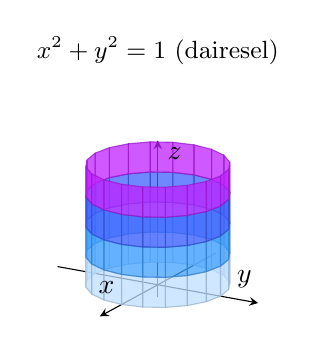
\begin{tikzpicture}
\begin{axis}[width=5.6cm,view={120}{25},axis lines=center,ticks=none,
  xlabel=$x$,ylabel=$y$,zlabel=$z$,colormap/cool,
  xmin=-1.6,xmax=1.6,ymin=-1.6,ymax=1.6,zmin=-0.2,zmax=2.4,
  title={\small $x^2+y^2=1$ (dairesel)}]
\addplot3[surf,shader=faceted,opacity=0.75,z buffer=sort,domain=0:360,y domain=0:2,samples=21,samples y=5]
  ({cos(x)},{sin(x)},{y});
\end{axis}
\end{tikzpicture}\qquad
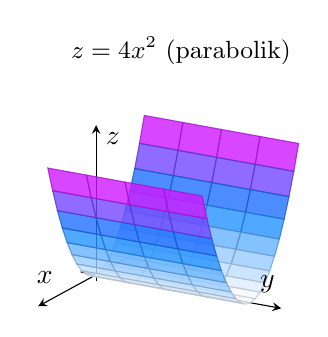
\begin{tikzpicture}
\begin{axis}[width=5.6cm,view={120}{25},axis lines=center,ticks=none,
  xlabel=$x$,ylabel=$y$,zlabel=$z$,colormap/cool,
  xmin=-1.2,xmax=1.2,ymin=-0.2,ymax=2.4,zmin=-0.2,zmax=4.5,
  title={\small $z=4x^2$ (parabolik)}]
\addplot3[surf,shader=faceted,opacity=0.8,domain=-1:1,y domain=0:2,samples=21,samples y=5]
  {4*x^2};
\end{axis}
\end{tikzpicture}
\end{center}

\begin{bilgi}[``Silindir'' kelimesi hakkında]
Günlük dilde ``silindir'' dairesel silindir demektir; matematikte ise dayanak eğrisi parabol, hiperbol, elips, hatta sinüs eğrisi olabilir. Örneğin $z=\sin y$ dalgalı bir oluk biçimli yüzeydir ($Ox$ eksenine paralel silindir). Düzlem de bir silindir sayılabilir: dayanak eğrisi doğru olan silindir.
\end{bilgi}

%======================================================================
\subsection{Kuadratik yüzeyler}

\begin{tanim}[Kuadratik (ikinci dereceden) yüzey]
$x,y,z$ cinsinden ikinci dereceden bir denklemin grafiğine \textbf{kuadratik yüzey} denir:
\[ Ax^2+By^2+Cz^2+Dxy+Exz+Fyz+Gx+Hy+Iz+J=0 . \]
Öteleme ve döndürme ile bu denklem standart biçimlerden birine getirilebilir. Bu derste karışık terimler ($xy$, $xz$, $yz$) olmayan durumla ilgileneceğiz; o zaman \emph{kareye tamamlama} (öteleme) yeterlidir.
\end{tanim}

\subsubsection{İzler (kesitler) yöntemi}

Bir yüzeyi kabaca çizmenin en etkili yolu, onu koordinat düzlemlerine paralel düzlemlerle kesip kesit eğrilerine (\textbf{izlere}) bakmaktır: $z=k$, $y=k$, $x=k$ düzlemleriyle arakesitler. Her iz, düzlemde tanıdığımız bir eğridir (elips, hiperbol, parabol, doğru çifti). Birkaç izi üst üste yerleştirince yüzeyin şekli ortaya çıkar.

\begin{tahta}[\foto{IMG-20261015-WA0043}]
Konu~4'teki $f(x,y)=x^2+y^2$ örneğinde $x^2+y^2=c$ seviye eğrileri $c=1,4,9$ için yarıçapları $1,2,3$ olan iç içe çemberler olarak çizilmiş, yanında da yatay çember kesitli $z=x^2+y^2$ yüzeyi gösterilmişti. Bu tam olarak izler yönteminin $z=k$ izleridir.
\end{tahta}
\begin{bilgi}[Çizim notu]
O fotoğraftaki yüzey düz kenarlarla, koni gibi çizilmiş. $z=x^2+y^2$ bir paraboloiddir; $x=0$ izi $z=y^2$ parabolü olduğu için kenarları \emph{eğridir} (kâse biçimi). Düz kenarlı yüzey $z=\sqrt{x^2+y^2}$ konisi olurdu.
\end{bilgi}

\begin{soru}[Örnek 15: izlerle tanıma]
$z=4x^2+y^2$ yüzeyinin izlerini bularak şeklini belirleyiniz.
\end{soru}
\begin{cevap}
\begin{itemize}
  \item $z=k$: $4x^2+y^2=k$. $k>0$ için elips ($\frac{x^2}{k/4}+\frac{y^2}{k}=1$), $k=0$ için yalnız orijin, $k<0$ için boş.
  \item $x=k$: $z=y^2+4k^2$, yukarı açılan parabol.
  \item $y=k$: $z=4x^2+k^2$, yukarı açılan parabol.
\end{itemize}
Yatay kesitler elips, dikey kesitler parabol $\Rightarrow$ tepe noktası orijinde, $Oz$ ekseni boyunca yukarı açılan \textbf{eliptik paraboloid}.
\end{cevap}

\subsubsection{Küre (kısaca)}

Konu~1'de gördüğümüz $M(a,b,c)$ merkezli, $r$ yarıçaplı küre $(x-a)^2+(y-b)^2+(z-c)^2=r^2$, aşağıdaki elipsoidin üç yarı ekseni eşit ($a=b=c=r$) olan özel hâlidir. Genel biçim $x^2+y^2+z^2+Dx+Ey+Fz+G=0$ kareye tamamlanarak merkez ve yarıçap bulunur; bütün kesitler çemberdir.

\subsubsection{Elipsoid}

\begin{tanim}[Elipsoid]
Koordinat düzlemleriyle arakesitleri elips olan yüzeye \textbf{elipsoid} denir:
\[ \frac{x^2}{a^2}+\frac{y^2}{b^2}+\frac{z^2}{c^2}=1\qquad(a,b,c>0). \]
\end{tanim}
\begin{itemize}
  \item Koordinat düzlemlerine göre simetriktir (her değişken kare olarak geçer); eksenleri $(\mp a,0,0)$, $(0,\mp b,0)$, $(0,0,\mp c)$ noktalarında keser.
  \item İzler: $z=k$ için $\frac{x^2}{a^2}+\frac{y^2}{b^2}=1-\frac{k^2}{c^2}$; $|k|<c$ ise elips, $|k|=c$ ise tek nokta, $|k|>c$ ise boş. Diğer izler de elipstir. Yüzey $|x|\le a$, $|y|\le b$, $|z|\le c$ kutusunun içindedir.
  \item $z$ çekilirse $z=\mp c\sqrt{1-\frac{x^2}{a^2}-\frac{y^2}{b^2}}$: $+$ işaret \textbf{üst yarı}, $-$ işaret \textbf{alt yarı} elipsoidi verir (her biri bir fonksiyon grafiğidir).
\end{itemize}

\begin{tahta}[\foto{IMG-20261015-WA0043}, \foto{IMG-20261023-WA0063}, \foto{IMG-20261022-WA0049}, \foto{IMG-20261108-WA0097}]
``Elipsoid: Koordinat düzlemleriyle arakesitleri elips olan yüzeylere denir. $\frac{x^2}{a^2}+\frac{y^2}{b^2}+\frac{z^2}{c^2}=1$. Bu yüzey koordinat düzlemlerine göre simetriktir; eksenleri $(\mp a,0,0)$, $(0,\mp b,0)$ ve $(0,0,\mp c)$ noktalarında keser. $z=c\sqrt{\cdots}$ üst elipsoid, $z=-c\sqrt{\cdots}$ alt elipsoid.''
(15.10 tahtasında ``koordinat düzlemine'' tekil yazılmıştı; doğrusu ``koordinat düzlemlerine''.)
\end{tahta}

\subsubsection{Hiperboloidler}

\begin{tanim}[Tek ve çift kanatlı hiperboloid]
\[ \textbf{Tek kanatlı:}\ \ \frac{x^2}{a^2}+\frac{y^2}{b^2}-\frac{z^2}{c^2}=1,\qquad
   \textbf{Çift kanatlı:}\ \ \frac{x^2}{a^2}+\frac{y^2}{b^2}-\frac{z^2}{c^2}=-1 . \]
Çift kanatlı olan $-\frac{x^2}{a^2}-\frac{y^2}{b^2}+\frac{z^2}{c^2}=1$ biçiminde de yazılır. Her ikisinde de \textbf{eksen}, işareti farklı olan değişkenin eksenidir (burada $Oz$).
\end{tanim}

\begin{tahta}[\foto{IMG-20261022-WA0049}, \foto{IMG-20261108-WA0097}, \foto{IMG-20261108-WA0096}]
``Bir hiperbolün yedek ekseni etrafında döndürülmesiyle tek kanatlı, asal ekseni etrafında döndürülmesiyle iki kanatlı hiperboloid elde edilir.'' Çizimler: kum saati biçimli tek kanatlı hiperboloid (``$z=0$'da elips, $x=0$'da hiperbol''); $z$ ekseni üzerinde biri yukarı biri aşağı açılan iki kâseden oluşan çift kanatlı hiperboloid (``$-c<z<c$ aralığında yüzey yok'').
\end{tahta}

\textbf{Tek kanatlı hiperboloidin izleri:} $z=k$ için $\frac{x^2}{a^2}+\frac{y^2}{b^2}=1+\frac{k^2}{c^2}$, \emph{her} $k$ için elips; en küçüğü $z=0$'daki ``bel'' elipsidir ve $|k|$ büyüdükçe büyür. $x=0$ için $\frac{y^2}{b^2}-\frac{z^2}{c^2}=1$ hiperbolü, $y=0$ için de hiperbol. Yüzey tek parçadır.

\textbf{Çift kanatlı hiperboloidin izleri:} $z=k$ için $\frac{x^2}{a^2}+\frac{y^2}{b^2}=\frac{k^2}{c^2}-1$; bu yalnız $|k|\ge c$ iken anlamlıdır. Bu yüzden $-c<z<c$ şeridinde yüzeyin hiçbir noktası yoktur; yüzey $z\ge c$ ve $z\le-c$ bölgelerinde iki ayrı parçadan (kanattan) oluşur, tepe noktaları $(0,0,\pm c)$'dir. $x=0$ ve $y=0$ izleri hiperboldür.

\textbf{Döndürme yorumu ($a=b$ iken):} $xz$-düzlemindeki $\frac{x^2}{a^2}-\frac{z^2}{c^2}=1$ hiperbolünün asal ekseni $Ox$, yedek (sanal) ekseni $Oz$'dir. Bu hiperbolü yedek ekseni $Oz$ etrafında döndürürsek $\frac{x^2+y^2}{a^2}-\frac{z^2}{c^2}=1$ tek kanatlı hiperboloidi; $\frac{z^2}{c^2}-\frac{x^2}{a^2}=1$ hiperbolünü asal ekseni $Oz$ etrafında döndürürsek çift kanatlı hiperboloidi elde ederiz. $a\neq b$ ise yüzeyler döndürme yüzeyi değildir ama şekil aynıdır.

\begin{center}
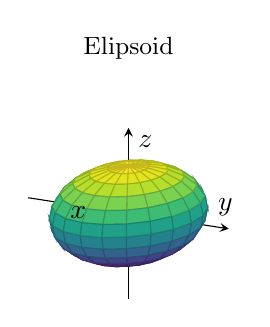
\begin{tikzpicture}
\begin{axis}[width=5.6cm,view={120}{20},axis lines=center,ticks=none,
  xlabel=$x$,ylabel=$y$,zlabel=$z$,colormap/viridis,
  xmin=-2.4,xmax=2.4,ymin=-2.4,ymax=2.4,zmin=-1.8,zmax=1.8,
  title={\small Elipsoid}]
\addplot3[surf,shader=faceted,z buffer=sort,domain=0:360,y domain=-90:90,samples=21,samples y=13]
  ({2*cos(y)*cos(x)},{1.5*cos(y)*sin(x)},{sin(y)});
\end{axis}
\end{tikzpicture}\qquad
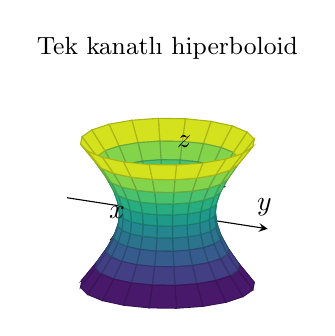
\begin{tikzpicture}
\begin{axis}[width=5.6cm,view={120}{20},axis lines=center,ticks=none,
  xlabel=$x$,ylabel=$y$,zlabel=$z$,colormap/viridis,
  xmin=-2.4,xmax=2.4,ymin=-2.4,ymax=2.4,zmin=-1.8,zmax=1.8,
  title={\small Tek kanatlı hiperboloid}]
\addplot3[surf,shader=faceted,z buffer=sort,domain=0:360,y domain=-1.2:1.2,samples=21,samples y=11]
  ({cosh(y)*cos(x)},{cosh(y)*sin(x)},{sinh(y)});
\end{axis}
\end{tikzpicture}
\end{center}
\begin{center}
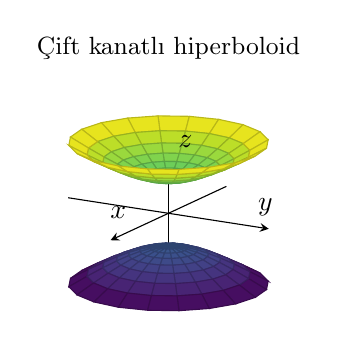
\begin{tikzpicture}
\begin{axis}[width=5.6cm,view={120}{20},axis lines=center,ticks=none,
  xlabel=$x$,ylabel=$y$,zlabel=$z$,colormap/viridis,
  xmin=-2.2,xmax=2.2,ymin=-2.2,ymax=2.2,zmin=-2.6,zmax=2.6,
  title={\small Çift kanatlı hiperboloid}]
\addplot3[surf,shader=faceted,z buffer=sort,domain=0:360,y domain=0:1.4,samples=21,samples y=9]
  ({sinh(y)*cos(x)},{sinh(y)*sin(x)},{cosh(y)});
\addplot3[surf,shader=faceted,z buffer=sort,domain=0:360,y domain=0:1.4,samples=21,samples y=9]
  ({sinh(y)*cos(x)},{sinh(y)*sin(x)},{-cosh(y)});
\end{axis}
\end{tikzpicture}\qquad
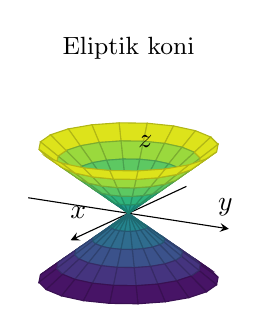
\begin{tikzpicture}
\begin{axis}[width=5.6cm,view={120}{20},axis lines=center,ticks=none,
  xlabel=$x$,ylabel=$y$,zlabel=$z$,colormap/viridis,
  xmin=-1.8,xmax=1.8,ymin=-1.8,ymax=1.8,zmin=-1.8,zmax=1.8,
  title={\small Eliptik koni}]
\addplot3[surf,shader=faceted,z buffer=sort,domain=0:360,y domain=-1.4:1.4,samples=21,samples y=11]
  ({y*cos(x)},{y*sin(x)},{y});
\end{axis}
\end{tikzpicture}
\end{center}

\subsubsection{Eliptik koni}

\begin{tanim}[Koni]
Sabit bir $T$ noktasından (tepe) geçen ve bir eğriyi kesen doğrunun hareketiyle oluşan yüzeye \textbf{koni} denir. Tepesi orijinde, ekseni $Oz$ olan eliptik koni:
\[ \frac{z^2}{c^2}=\frac{x^2}{a^2}+\frac{y^2}{b^2}\quad\Longrightarrow\quad z=\mp c\sqrt{\frac{x^2}{a^2}+\frac{y^2}{b^2}} . \]
$z=c\sqrt{\cdots}$ üst koni, $z=-c\sqrt{\cdots}$ alt konidir.
\end{tanim}
\begin{itemize}
  \item $z=k\neq0$: $\frac{x^2}{a^2}+\frac{y^2}{b^2}=\frac{k^2}{c^2}$ elips ($a=b$ ise çember); $k=0$: yalnız tepe noktası.
  \item $x=0$: $\frac{z^2}{c^2}=\frac{y^2}{b^2}$, yani $z=\pm\frac cb\,y$ \textbf{doğru çifti}; $y=0$ için de doğru çifti. $x=k\neq0$ izleri hiperboldür.
  \item Koni, tek ve çift kanatlı hiperboloidlerin ``arasındaki'' sınır durumudur: sağ taraf $1$, $0$, $-1$ olarak değişirken tek kanatlı hiperboloid $\to$ koni $\to$ çift kanatlı hiperboloid.
\end{itemize}

\begin{tahta}[\foto{IMG-20261022-WA0052}, \foto{IMG-20261108-WA0096}]
``Koni: Sabit bir $T$ noktasından geçen ve bir eğriyi kesen doğrunun oluşturduğu yüzeye denir. $\frac{z^2}{c^2}=\frac{x^2}{a^2}+\frac{y^2}{b^2}\to z=\mp c\sqrt{\frac{x^2}{a^2}+\frac{y^2}{b^2}}$.'' Çizim: tepe noktası orijinde, yukarı ve aşağı açılan çift koni ``(Tepe orijinde)''.
\end{tahta}

\subsubsection{Eliptik paraboloid}

\begin{tanim}[Eliptik paraboloid]
\[ z=\frac{x^2}{a^2}+\frac{y^2}{b^2}\qquad\text{(genel olarak } \tfrac{z}{c}=\tfrac{x^2}{a^2}+\tfrac{y^2}{b^2}\text{)} . \]
$z=k$ ($k>0$) düzlemleriyle arakesitleri elips olduğu için bu yüzeye \textbf{eliptik paraboloid} denir. $x=k$ ve $y=k$ izleri paraboldür. $c>0$ iken tepe noktası orijinde, yukarı açılan bir kâsedir.
\end{tanim}

\begin{tahta}[\foto{IMG-20261022-WA0050}, \foto{IMG-20261108-WA0096}]
``Parabolün simetri ekseni etrafında döndürülmesiyle elde edilen yüzeye paraboloid denir. Bu yüzeyin $z=c$ $(c>0)$ düzlemleriyle arakesiti bir elips olduğundan bu yüzeye eliptik paraboloid denir.'' (22.10 tahtasında başlık önce ``Hiper\ldots'' diye başlanıp düzeltilmiş ve ``Eliptoik'' diye yazılmıştı; doğrusu ``Eliptik''.)
\end{tahta}
\begin{bilgi}[Dönel paraboloid]
Bir parabolü simetri ekseni etrafında döndürmek, yalnızca $a=b$ olan \textbf{dönel paraboloidi} ($z=\frac{x^2+y^2}{a^2}$, yatay kesitleri çember) verir. $a\neq b$ iken yüzey bir döndürme yüzeyi değildir; kesitleri gerçek elipslerdir. Tahtadaki tanım bu nedenle önce dönel paraboloidi anlatıp sonra adı ``eliptik''e genişletiyor.
\end{bilgi}

\subsubsection{Hiperbolik paraboloid (eyer yüzeyi)}

\begin{tanim}[Hiperbolik paraboloid]
\[ \frac{z}{c}=\frac{x^2}{a^2}-\frac{y^2}{b^2}\qquad\text{(eyer / semer yüzeyi)}. \]
\end{tanim}
\begin{itemize}
  \item $z=k$: $\frac{x^2}{a^2}-\frac{y^2}{b^2}=\frac kc$ \textbf{hiperbol}ler ($k>0$ ve $k<0$ için farklı eksenlere açılır); $k=0$ için $y=\pm\frac ba x$ doğru çifti.
  \item $y=k$: $z=\frac{c}{a^2}x^2-\frac{ck^2}{b^2}$, yukarı açılan parabol ($c>0$).
  \item $x=k$: $z=\frac{ck^2}{a^2}-\frac{c}{b^2}y^2$, aşağı açılan parabol.
  \item Orijin bir \textbf{eyer noktasıdır}: $x$ yönünde yürüyünce orijin en alçak nokta, $y$ yönünde yürüyünce en yüksek noktadır. Bu nokta Konu~5--6'da ekstremum testlerinde tekrar karşımıza çıkacak.
\end{itemize}

\begin{tahta}[\foto{IMG-20261022-WA0052}, \foto{IMG-20261108-WA0095}]
``Hiperbolik paraboloid: $\frac zc=\frac{x^2}{a^2}-\frac{y^2}{b^2}$ (eyer yüzeyi).'' Tel kafes (ağ) biçiminde eyer çizimi.
(Bazı kitaplarda standart biçim $\frac zc=\frac{y^2}{b^2}-\frac{x^2}{a^2}$ olarak verilir; bu yalnızca yönelim farkıdır, yüzey aynı türdendir.)
\end{tahta}

\begin{center}
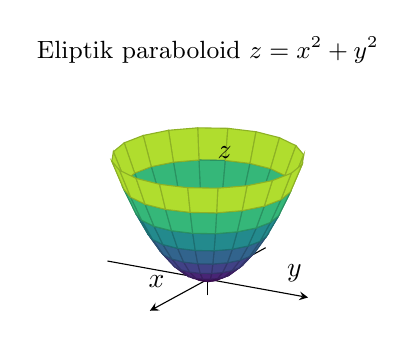
\begin{tikzpicture}
\begin{axis}[width=5.6cm,view={120}{25},axis lines=center,ticks=none,
  xlabel=$x$,ylabel=$y$,zlabel=$z$,colormap/viridis,
  xmin=-1.8,xmax=1.8,ymin=-1.8,ymax=1.8,zmin=-0.3,zmax=2.6,
  title={\small Eliptik paraboloid $z=x^2+y^2$}]
\addplot3[surf,shader=faceted,z buffer=sort,domain=0:360,y domain=0:1.5,samples=21,samples y=9]
  ({y*cos(x)},{y*sin(x)},{y^2});
\end{axis}
\end{tikzpicture}\qquad
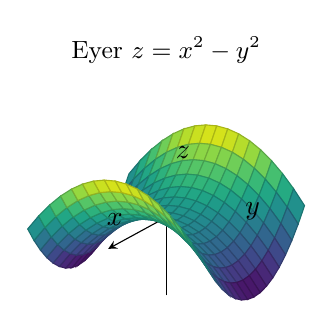
\begin{tikzpicture}
\begin{axis}[width=5.6cm,view={120}{25},axis lines=center,ticks=none,
  xlabel=$x$,ylabel=$y$,zlabel=$z$,colormap/viridis,
  xmin=-1.6,xmax=1.6,ymin=-1.6,ymax=1.6,zmin=-2.4,zmax=2.4,
  title={\small Eyer $z=x^2-y^2$}]
\addplot3[surf,shader=faceted,domain=-1.4:1.4,y domain=-1.4:1.4,samples=17]
  {x^2-y^2};
\end{axis}
\end{tikzpicture}
\end{center}

\subsubsection{Standart biçimler ve tanıma rehberi}

\begin{center}
\begin{tabular}{l l l}
\toprule
Yüzey & Standart denklem ($Oz$ ekseni) & İzler \\
\midrule
Elipsoid & $\frac{x^2}{a^2}+\frac{y^2}{b^2}+\frac{z^2}{c^2}=1$ & hepsi elips \\
Tek kanatlı hiperboloid & $\frac{x^2}{a^2}+\frac{y^2}{b^2}-\frac{z^2}{c^2}=1$ & $z=k$: elips; $x,y=k$: hiperbol \\
Çift kanatlı hiperboloid & $\frac{x^2}{a^2}+\frac{y^2}{b^2}-\frac{z^2}{c^2}=-1$ & $z=k$ ($|k|>c$): elips; diğer: hiperbol \\
Eliptik koni & $\frac{z^2}{c^2}=\frac{x^2}{a^2}+\frac{y^2}{b^2}$ & $z=k$: elips; $x,y=0$: doğru çifti \\
Eliptik paraboloid & $\frac{z}{c}=\frac{x^2}{a^2}+\frac{y^2}{b^2}$ & $z=k$: elips; $x,y=k$: parabol \\
Hiperbolik paraboloid & $\frac{z}{c}=\frac{x^2}{a^2}-\frac{y^2}{b^2}$ & $z=k$: hiperbol; $x,y=k$: parabol \\
Silindir & bir değişken eksik & eksik değişken yönünde sabit \\
\bottomrule
\end{tabular}
\end{center}

\begin{teorem}[Hızlı tanıma]
Denklemi (gerekirse kareye tamamlayarak) standart biçime getirin, sonra:
\begin{enumerate}
  \item Bir değişken hiç yoksa $\to$ \textbf{silindir} (o eksene paralel).
  \item Üç değişken de kare ve sabit terim var: hepsi aynı işaretli $\to$ \textbf{elipsoid}; biri farklı işaretli $\to$ \textbf{hiperboloid}. Hiperboloid için $=1$ biçiminde yazınca \emph{bir} eksi işaret varsa \textbf{tek kanatlı}, \emph{iki} eksi işaret varsa \textbf{çift kanatlı}dır. Eksen, işareti ``yalnız kalan'' değişkenin eksenidir.
  \item Üç değişken kare, sabit terim yok (sağ taraf $0$) ve işaretler karışık $\to$ \textbf{koni}.
  \item İki değişken kare, biri birinci dereceden $\to$ \textbf{paraboloid}: karelerin işaretleri aynıysa \textbf{eliptik}, farklıysa \textbf{hiperbolik}. Eksen, birinci dereceden değişkenin eksenidir.
\end{enumerate}
\end{teorem}

\subsubsection{Genel kuadratik denklemi kareye tamamlayarak tanıma}

\begin{bilgi}[Derste tahtada görülmedi, kaynaklardan eklendi]
Karışık terimi olmayan $Ax^2+By^2+Cz^2+Gx+Hy+Iz+J=0$ denkleminde her değişken için kareye tamamlanır: $x^2-2px=(x-p)^2-p^2$. Böylece yüzey, merkezi/tepesi $(p,q,r)$ noktasına ötelenmiş bir standart yüzey olarak tanınır (Konu~1'de küre denkleminde yaptığımız işlemin aynısı).
\end{bilgi}

\begin{soru}[Örnek 16 (kaynaklardan)]
$x^2+2z^2-6x-y+10=0$ yüzeyini tanıyınız.
\end{soru}
\begin{cevap}
$x$ için kareye tamamlayalım: $x^2-6x=(x-3)^2-9$. Denklem
\[ (x-3)^2-9+2z^2-y+10=0\ \Longrightarrow\ y-1=(x-3)^2+2z^2 . \]
İki değişken ($x$, $z$) kare ve aynı işaretli, $y$ birinci dereceden $\Rightarrow$ \textbf{eliptik paraboloid}. Tepe noktası $(3,1,0)$, ekseni $Oy$'ye paralel ($x=3,\ z=0$ doğrusu), $+y$ yönünde açılır. $y=k$ ($k>1$) izleri $(x-3)^2+2z^2=k-1$ elipsleridir.
\end{cevap}

\begin{soru}[Örnek 17 (kaynaklardan)]
$x^2+y^2-z^2-4x+6y+2z+8=0$ yüzeyini tanıyınız.
\end{soru}
\begin{cevap}
Kareye tamamlama: $x^2-4x=(x-2)^2-4$, $y^2+6y=(y+3)^2-9$, $-(z^2-2z)=-(z-1)^2+1$. Yerine yazarsak
\[ (x-2)^2-4+(y+3)^2-9-(z-1)^2+1+8=0\ \Longrightarrow\ (x-2)^2+(y+3)^2-(z-1)^2=4, \]
\[ \frac{(x-2)^2}{4}+\frac{(y+3)^2}{4}-\frac{(z-1)^2}{4}=1 . \]
Sağ taraf $1$ iken \emph{bir} eksi işaret $\Rightarrow$ \textbf{tek kanatlı hiperboloid}; merkezi $(2,-3,1)$, ekseni $Oz$'ye paralel. $a=b=2$ olduğundan dönel hiperboloiddir; bel çemberi $z=1$ düzleminde, yarıçapı $2$.
\end{cevap}

%======================================================================
\subsection{Kaynak kitaplardan ek örnekler}

\begin{soru}[\ekal Ek örnek 1: aykırı doğrular]
$d_1:\ x=1+t,\ y=-2+3t,\ z=4-t$ ve $d_2:\ x=2s,\ y=3+s,\ z=-3+4s$ doğrularının paralel, kesişen ya da aykırı olduğunu belirleyiniz; aykırı ise aralarındaki uzaklığı bulunuz.
\end{soru}
\begin{cevap}
Doğrultmanlar $\mathbf v=(1,3,-1)$, $\mathbf u=(2,1,4)$; oranlar $\frac12\neq\frac31$ olduğundan paralel değiller.

Kesişme: $1+t=2s$ ve $-2+3t=3+s$. İlkinden $t=2s-1$; ikincide $-2+6s-3=3+s\Rightarrow5s=8$, $s=\frac85$, $t=\frac{11}{5}$. Üçüncü bileşen: $4-t=\frac95$, $-3+4s=\frac{17}{5}$; eşit değil $\Rightarrow$ kesişmezler. Doğrular \textbf{aykırıdır}.

Uzaklık: $P_1(1,-2,4)$, $P_2(0,3,-3)$, $\overrightarrow{P_1P_2}=(-1,5,-7)$.
\[ \mathbf v\times\mathbf u=\begin{vmatrix}\mathbf i&\mathbf j&\mathbf k\\1&3&-1\\2&1&4\end{vmatrix}=(12+1,\ -(4+2),\ 1-6)=(13,-6,-5), \]
\[ d=\frac{|(-1)(13)+5(-6)+(-7)(-5)|}{\sqrt{169+36+25}}=\frac{|-13-30+35|}{\sqrt{230}}=\frac{8}{\sqrt{230}}\approx0{,}53 . \]
\end{cevap}

\begin{soru}[\ekal Ek örnek 2: kesişen doğrular]
$d_1:\ x=1+t,\ y=2-t,\ z=3+2t$ ve $d_2:\ x=1+s,\ y=-1+2s,\ z=6-s$ doğrularının kesişip kesişmediğini belirleyiniz; kesişiyorlarsa kesim noktasını ve aralarındaki açıyı bulunuz.
\end{soru}
\begin{cevap}
$x$: $1+t=1+s\Rightarrow t=s$. $y$: $2-t=-1+2s=-1+2t\Rightarrow t=1$, $s=1$. $z$: $3+2(1)=5$ ve $6-1=5$ \checkmark. Doğrular \textbf{kesişir}; kesim noktası $(2,1,5)$.

Açı: $\mathbf v=(1,-1,2)$, $\mathbf u=(1,2,-1)$, $\mathbf v\cdot\mathbf u=1-2-2=-3$, $\|\mathbf v\|=\|\mathbf u\|=\sqrt6$:
$\cos\theta=\frac{|-3|}{6}=\frac12\Rightarrow\theta=60^\circ$.
\end{cevap}

\begin{soru}[\ekal Ek örnek 3: düzlemler arası açı]
$x+y+z=1$ ve $x-2y+3z=1$ düzlemleri arasındaki açıyı bulunuz.
\end{soru}
\begin{cevap}
$\mathbf n_1=(1,1,1)$, $\mathbf n_2=(1,-2,3)$, $\mathbf n_1\cdot\mathbf n_2=1-2+3=2$, $\|\mathbf n_1\|=\sqrt3$, $\|\mathbf n_2\|=\sqrt{14}$:
\[ \cos\theta=\frac{2}{\sqrt3\sqrt{14}}=\frac{2}{\sqrt{42}}\approx0{,}309\ \Rightarrow\ \theta\approx72^\circ . \]
\end{cevap}

\begin{soru}[\ekal Ek örnek 4: paralel düzlemler arası uzaklık]
$10x+2y-2z=5$ ve $5x+y-z=1$ düzlemleri arasındaki uzaklığı bulunuz.
\end{soru}
\begin{cevap}
Normaller $(10,2,-2)=2(5,1,-1)$; düzlemler paralel. Formülü kullanmak için \emph{aynı katsayılarla} yazalım: ikinci denklemi $2$ ile çarparsak $10x+2y-2z-2=0$; birincisi $10x+2y-2z-5=0$. Böylece $D_1=-5$, $D_2=-2$:
\[ d=\frac{|D_2-D_1|}{\sqrt{100+4+4}}=\frac{3}{\sqrt{108}}=\frac{3}{6\sqrt3}=\frac{\sqrt3}{6}\approx0{,}289 . \]
(Kontrol: birinci düzlemden $K(\frac12,0,0)$ alıp ikinciye uzaklığı: $\frac{|5/2-1|}{\sqrt{27}}=\frac{3/2}{3\sqrt3}=\frac{\sqrt3}{6}$ \checkmark.)
\end{cevap}

\begin{soru}[\ekal Ek örnek 5: iki düzleme paralel doğru]
$P(1,-1,2)$ noktasından geçen ve $x+y-z=1$ ile $2x-y+3z=4$ düzlemlerinin ikisine de paralel olan doğrunun denklemini yazınız.
\end{soru}
\begin{cevap}
Doğru her iki düzleme paralelse doğrultmanı iki normale de diktir: $\mathbf v=\mathbf n_1\times\mathbf n_2$.
\[ \mathbf v=\begin{vmatrix}\mathbf i&\mathbf j&\mathbf k\\1&1&-1\\2&-1&3\end{vmatrix}=\big(3-1,\ -(3+2),\ -1-2\big)=(2,-5,-3). \]
\[ \frac{x-1}{2}=\frac{y+1}{-5}=\frac{z-2}{-3}. \]
Kontrol: $\mathbf v\cdot\mathbf n_1=2-5+3=0$, $\mathbf v\cdot\mathbf n_2=4+5-9=0$ \checkmark.
\end{cevap}

\begin{soru}[\ekal Ek örnek 6: silindiri tanıma]
$y^2+z^2=9$ ve $x=y^2$ yüzeylerini tanıyınız.
\end{soru}
\begin{cevap}
$y^2+z^2=9$ denkleminde $x$ yok $\Rightarrow$ $Ox$ eksenine paralel silindir; dayanak eğrisi $yz$-düzleminde yarıçapı $3$ olan çember: ekseni $Ox$ olan \textbf{dairesel silindir}.

$x=y^2$ denkleminde $z$ yok $\Rightarrow$ $Oz$'ye paralel silindir; dayanak eğrisi $xy$-düzleminde $x=y^2$ parabolü: \textbf{parabolik silindir} (dikey duran bir oluk).
\end{cevap}

\begin{soru}[\ekal Ek örnek 7: çift kanatlı hiperboloid]
$4x^2-y^2+2z^2+4=0$ yüzeyini tanıyınız.
\end{soru}
\begin{cevap}
$-4$'e bölersek $-x^2+\frac{y^2}{4}-\frac{z^2}{2}=1$. Sağ taraf $1$ iken \emph{iki} eksi işaret $\Rightarrow$ \textbf{çift kanatlı hiperboloid}; yalnız kalan pozitif değişken $y$ olduğundan ekseni $Oy$'dir. $y=k$ izleri $x^2+\frac{z^2}{2}=\frac{k^2}{4}-1$, yalnız $|k|\ge2$ için var: yüzey $-2<y<2$ şeridinde boştur, tepe noktaları $(0,\pm2,0)$.
\end{cevap}

%======================================================================
\subsection{Sık yapılan hatalar}

\begin{dikkat}
\begin{itemize}
  \item \textbf{Uzayda doğruyu tek denklemle yazmak.} $3x-2y+1=0$ uzayda bir düzlemdir; doğru için iki denklem (ya da parametrik/kartezyen biçim) gerekir (Örnek~1).
  \item \textbf{Paydada sıfıra bölmek.} Doğrultman parametresi $0$ ise o değişken sabittir: $\mathbf v=(2,3,0)$ ise $z=z_0$ yazılır.
  \item \textbf{Normal ile doğrultmanı karıştırmak.} Düzlemin $x,y,z$ katsayıları \emph{normaldir}, doğrunun paydaları \emph{doğrultmandır}. Doğru düzleme dikse $\mathbf v\parallel\mathbf n$, paralelse $\mathbf v\perp\mathbf n$ (tersini yazmak çok yaygın bir hatadır).
  \item \textbf{Doğrunun noktasını yanlış işaretle almak.} $\frac{z+1}{6}$ ifadesinde $z_0=-1$'dir, $+1$ değil.
  \item \textbf{Paralel düzlem uzaklığını katsayıları eşitlemeden hesaplamak.} $|D_2-D_1|$ formülü yalnız $A,B,C$ aynı iken geçerlidir (Ek örnek 4).
  \item \textbf{$D$'yi yanlış taraftan okumak.} $2x+2y+2z=5$ için $D=-5$'tir; önce $Ax+By+Cz+D=0$ biçimine getirin.
  \item \textbf{Açıda mutlak değeri unutmak.} Doğrular/düzlemler arası açı istenirken dar açı verilir; $\cos\theta<0$ çıkarsa $180^\circ-\theta$ alın.
  \item \textbf{Paralellik testini $aA+bB+cC=0$ ile bitirmek.} Doğru düzlemin içinde de olabilir; bir noktasını düzlemde deneyin.
  \item \textbf{Sağlama yapmamak.} Bulunan düzlemin verilen noktalardan geçtiğini, kesim noktasının hem doğruyu hem düzlemi sağladığını kontrol edin (Örnek~7'deki tahta hatası böyle yakalanır).
  \item \textbf{Hiperboloidleri karıştırmak.} $=1$ biçiminde bir eksi: tek kanatlı; iki eksi: çift kanatlı. Sağ taraf $0$ ise koni.
  \item \textbf{Paraboloidi koni gibi çizmek.} $z=x^2+y^2$ kâse biçimlidir; $z=\sqrt{x^2+y^2}$ konidir.
\end{itemize}
\end{dikkat}

%======================================================================
\subsection{Özet ve formül kutusu}

\begin{ozet}
\textbf{Doğru} ($A(x_0,y_0,z_0)$, $\mathbf v=(a,b,c)$):
\[ \overrightarrow{AP}=t\mathbf v;\quad x=x_0+at,\ y=y_0+bt,\ z=z_0+ct;\quad \frac{x-x_0}{a}=\frac{y-y_0}{b}=\frac{z-z_0}{c}. \]
$b=0$ ise $y=y_0$, $\frac{x-x_0}{a}=\frac{z-z_0}{c}$. İki noktadan geçen doğru: $\mathbf v=\overrightarrow{AB}$.

\textbf{İki doğru} ($\mathbf v=(a,b,c)$, $\mathbf u=(p,q,r)$): paralel $\frac ap=\frac bq=\frac cr$; dik $ap+bq+cr=0$;
$\cos\theta=\frac{|\mathbf u\cdot\mathbf v|}{\|\mathbf u\|\|\mathbf v\|}$; aykırı uzaklık $\frac{|\overrightarrow{P_1P_2}\cdot(\mathbf v\times\mathbf u)|}{\|\mathbf v\times\mathbf u\|}$.

\textbf{Nokta--doğru uzaklığı:} $\ell=\dfrac{\|\overrightarrow{AP}\times\mathbf v\|}{\|\mathbf v\|}$.

\textbf{Düzlem} ($P_0$, $\mathbf n=(A,B,C)$): $A(x-x_0)+B(y-y_0)+C(z-z_0)=0$, $Ax+By+Cz+D=0$.
Üç nokta: $\mathbf n=\overrightarrow{AB}\times\overrightarrow{AC}$ (determinant $=0$). Doğruya dik düzlem: $\mathbf n=\mathbf v$.

\textbf{İki düzlem:} paralel $\frac{A_1}{A_2}=\frac{B_1}{B_2}=\frac{C_1}{C_2}$ ($\neq\frac{D_1}{D_2}$); çakışık ($=\frac{D_1}{D_2}$); dik $A_1A_2+B_1B_2+C_1C_2=0$;
$\cos\theta=\frac{|\mathbf n_1\cdot\mathbf n_2|}{\|\mathbf n_1\|\|\mathbf n_2\|}$; arakesit doğrultmanı $\mathbf n_1\times\mathbf n_2$.

\textbf{Doğru--düzlem:} dik $\frac aA=\frac bB=\frac cC$; paralel (veya içinde) $aA+bB+cC=0$; $\sin\varphi=\frac{|\mathbf v\cdot\mathbf n|}{\|\mathbf v\|\|\mathbf n\|}$; kesim noktası: parametrik denklemi düzlemde yerine koy.

\textbf{Uzaklıklar:}
\[ d(P,\text{düzlem})=\frac{|Ax_0+By_0+Cz_0+D|}{\sqrt{A^2+B^2+C^2}},\qquad d(P_1,P_2)=\frac{|D_2-D_1|}{\sqrt{A^2+B^2+C^2}}. \]

\textbf{Silindir:} bir değişken eksik $\Rightarrow$ o eksene paralel silindir.

\textbf{Kuadratik yüzeyler} ($Oz$ ekseni):
\begin{center}
\begin{tabular}{l l}
\toprule
Elipsoid & $\frac{x^2}{a^2}+\frac{y^2}{b^2}+\frac{z^2}{c^2}=1$\\
Tek kanatlı hiperboloid & $\frac{x^2}{a^2}+\frac{y^2}{b^2}-\frac{z^2}{c^2}=1$\\
Çift kanatlı hiperboloid & $\frac{x^2}{a^2}+\frac{y^2}{b^2}-\frac{z^2}{c^2}=-1$\\
Eliptik koni & $\frac{z^2}{c^2}=\frac{x^2}{a^2}+\frac{y^2}{b^2}$\\
Eliptik paraboloid & $\frac zc=\frac{x^2}{a^2}+\frac{y^2}{b^2}$\\
Hiperbolik paraboloid (eyer) & $\frac zc=\frac{x^2}{a^2}-\frac{y^2}{b^2}$\\
\bottomrule
\end{tabular}
\end{center}
Tanıma: kareye tamamla $\to$ işaretleri say $\to$ izlere bak.
\end{ozet}

\end{document}
